% ------------------------------------
% Universidad de Costa Rica
% Facultad de Ingeniería
% Escuela de Ingeniería Eléctrica
% IE0499 - Proyecto Eléctrico
%
% PLANTILLA DEL TRABAJO ESCRITO
% ------------------------------------

% Tipo de documento
\documentclass[]{proyectoelectrico}

% A. PAQUETES Y MACROS ESPECIALES -------
% Aquellos que no están incluidos en la clase
% proyectoelectrico.cls

% -----------------------------------------
% OTROS PAQUETES E INSTRUCCIONES ESPECIALES
% -----------------------------------------

% Para insertar código fuente estilizado
\usepackage{listings}
    \lstset{basicstyle=\ttfamily,
            breaklines=true,
            numbers=left,
            numberstyle=\tiny,
            stepnumber=1,
            numbersep=6pt}

% Para insertar símbolos extraños
\usepackage{marvosym}

% Para insertar texto fútil
\usepackage{lipsum}

% Para dibujar matrices
%\usepackage{amsmath}

% NUEVAS INSTRUCCIONES

\newcommand{\EIEx}{\textsc{Escuela \Lightning~ Ingeniería Eléctrica}}

% Definición de algunos símbolos matemáticos
\newcommand{\me}{\mathrm{e}}
\newcommand{\mi}{\mathrm{i}}
\newcommand{\mj}{\mathrm{j}}
\newcommand{\md}{\mathrm{d}}

\usepackage{libertine}
%\usepackage{libertinust1math}
\usepackage[T1]{fontenc}
\renewcommand*{\ttdefault}{cmtt}

% B. DATOS ------------------------------
% Todos los nombres incluyen dos apellidos
% y acentos y signos de puntuación apropiados.

% Título del proyecto
\titulo{Implementación de mapeo y localización simultánea para un robot móvil con ruedas mecanum.}

%% Autor (nombre y carné)
\autor{Stuart Leal Quesada}
\carne{B53777}

% Profesor(a) guía
\guia{Ing. Federico Ruíz Ugalde, Dr.rer.nat}

% Profesores lectores
\lectorA{Ing. Israel Arbaiza, Lic.}
\lectorB{Ing. Fabián Abarca Calderón, M.Sc.}

% Fecha de entrega del trabajo escrito
\mes{4}
\ano{2018}

% ------------------------------------

%%%%%%%%%%%%%%%%%%%
\begin{document}
%%%%%%%%%%%%%%%%%%%

\frontmatter

% 1. PORTADA
\portada

% 2. HOJA DE APROBACIÓN
\aprobacion

% 3. RESUMEN (EN ESPAÑOL E INGLÉS)
% --------------------------------
%% EL RESUMEN
% ----------

\begin{resumen}{palabras, claves, separadas, por, coma}

Este es el resumen del trabajo. Tiene un máximo de 300 palabras y debe ajustarse a una sola página en este formato.

\lipsum[1-2]

\end{resumen}
%% EL RESUMEN EN INGLÉS
% --------------------

\begin{theabstract}{Title of the Project in English}{keywords, separated, by, a, comma}

This is a test of the abstract of the project. It should not have more than 300 words or exceed one page in this template (whichever happens first).

\lipsum[1-2]

\end{theabstract}

% El entorno 'theabstract' tiene el formato \begin{theabstract}{A} ...B... \end{theabstract} donde A es el título del proyecto traducido de inglés a español y B es el contenido, en inglés, del resumen. Se recomienda buscar ayuda calificada para la elaboración y/o revisión de este resumen.

% 4. DEDICATORIA
%% LA DEDICATORIA
% --------------

\begin{dedicatoria}
Dedicado a
\end{dedicatoria}

% 5. AGRADECIMIENTOS
%% LOS AGRADECIMIENTOS
% -------------------

\begin{agradecimientos}

\lipsum[5]

\end{agradecimientos}

% 6. TABLAS DE CONTENIDO, FIGURAS Y TABLAS
% ----------------------------------------
\tableofcontents
\listoffigures
\listoftables

% 7. NOMENCLATURA
% ---------------
% LA NOMENCLATURA
% ---------------

\mainmatter

% 8. CAPÍTULOS
% ------------
% ----------------------
  \chapter{Introducción}
% ----------------------
\label{C:introduccion}



%--------------------------------------------------------------------

La robótica es la ciencia de percibir y manipular el mundo físico através de dispositivos mecánicos controlados por computadoras \cite{Thrun2005}. Hasta hoy la robótica ha logrado perfeccionar los movimientos precisos milimétricamente, y las tareas repetitivas. Sin embargo, fuera de una línea de producción, estas ventajas no son útiles, por ejemplo en un hogar los ambientes son dinámicos y el robot por lo tanto debe poseer características cognitivas \cite{HelioAzevedoRenatoArcherITCenterandICM/USPJosePedroR.InstituteofMathematicalandComputerSciences2017}.

El laboratorio de investigación ARCOS-Lab (Autonomous Robots and Cognitive Systems) se enfoca primariamente en desarrollar e implementar nuevas técnicas en dispositivos mecánicos con el fin de satisfacer algunas de las necesidades mencionadas anteriormente.

Actualmente (2018) el ARCOS-Lab está trabajando en la construcción de un robot humanoide, el cuál se desea que pueda reconocer su ambiente, y realizar tareas dinámicas como cocinar. La navegación es uno de los aspectos más importantes que se debe desarrollar para cumplir el fin propuesto. Por lo tanto, el presente proyecto plantea implementar un algoritmo llamado SLAM (Simultaneous localization and mapping) en la navegación dos-dimensional de un robot omnidireccional con ruedas mecanum.

Actualmente, el ARCOS-Lab ha desarrollado varios prototipos de robots omnidireccionales. Sin embargo, a través de las iteraciones se han ido perfeccionando aspectos, cómo el diseño de la base, y las piezas necesarias para crear una base omnidireccional estable, robusta y diseñada con precisión.

De los primeros diseños que se realizó, el ensamble de la base se realizó en una base de madera en la cuál los montajes para los motores no se diseñaron con computadora. Esto causa problemas en los movimientos omnidireccionales del robot, por lo que el diseño de la base se debío realizar con una computadora, y cortar con precisión en una cortadora láser.

Este proyecto pretende ensamblar eléctricamente la base del carro omnidireccional, utilizando las piezas ya diseñadas, impresas, y cortadas, y dotarlo de la capacidad de navegación dos dimencional. Por lo tanto, viene a completar la posiblidad de que con este robot se realice navegación autónoma.

\newpage
\section{Alcance}
Se pretende implementar SLAM en robots pequeños denomindados ``\textit{mobile robots}'' dentro del contexto del ARCOS-Lab. Los mismos son plataformas de aproximadamente $50cm$ x $20cm$. Fueron contruidos para implementar los algoritmos de navegación, y realizar investigación en esta área, con el fin de perfeccionar el sistema que se utilizará para el robot humanoide. Las plataformas poseen en esencia el mismo sistema de ruedas omnidireccionales mecanum del robot humanoide.

En principio, es difícil experimentar con la base del robot humanoide desde un inicio. Primero está la limitación de que la misma plataforma está en un constante proceso de desarrollo, lo que quiere decir que se le hacen mejoras constantemente. Esto dificulta la disponibilidad de la base. Además, en los casos en que la plataforma se controle incorrectamente, los daños que pueda ocasionar a una persona o los objetos dentro del laboratorio son superiores a los que podrían ocasionar las plataformas más pequeñas.

El producto final de este proyecto eléctrico es proporcionar los diseños de código y ensamble, así como de conexiones eléctricas para los componentes existentes, para ensamblar un robot omnidireccional que listo para realizar navegación autónoma, por medio del sistema ROS (Robot Operating System).

\subsection{Equipo}
A continuación se hace una breve descripción del equipo principal utilizado para la construcción de las plataformas omnidireccionales utilizadas.

\begin{itemize}
\item \textit{Motores DC}: Los motores DC utilizados para cada una de las cuatro ruedas de la plataforma omnidireccional. Son motores de $12V$, con un consumo de aproximado $0.53A$ sin carga, y un codificador de cuadratura que produce 3415 pulsos por revolución. El motor logra alcanzar hasta 118rpm según la hoja de fabricante.
\item \textit{Roboclaw 2x15A}: Este controlador está diseñado para manejar dos motores DC de máximo 15A cada uno, por lo que se utilizarán dos de estos controladores para manejar los cuatro motores.
\item \textit{STM32F4}: Se necesita un controlador con capacidad de mandar los comandos de control hacia el Roboclaw para poder comandar la plataforma correctamente. Se utilizará un microcontrolador STM32F411-disco para esta tarea. La odemetría será calculada en este microcontrolador, en vez del Roboclaw para mayor precisión.
\item \textit{RaspBerry PI}: Se utiliza este microcontrolador, como la unidad de procesamiento principal en donde se controlarán los perifericos por medio del sistema de ROS. A esta tarjeta se conectará el Kinect y el Stm32F4.
\item \textit{Kinect 2}: Este será el sensor utilizado para la odometría visual. Será utilizado principalmente para generar la información del mapa, y posteriormente la ubicación del robot dentro del mismo mapa.
\end{itemize}

\subsection{Herramientas}
Se describen las herramientas que se utilizarán en el desarrollo del proyecto.

\begin{itemize}
\item \textit{ROS}: El desarollo e implentación de SLAM se realizará en ROS, puesto que es un sistema que permite la modularización de los diferentes componentes del robot. Facilita la conexión entre los diferentes perifericos. Posee librerías que contienen el código necesario para implementar SLAM.
\item \textit{Libopencm3}: Biblioteca para desarrollar el código en C del microcontrolador STM32F411.
\item \textit{Libopencm3-plus}: Biblioteca desarrollada por el Arcos-LAB que provee funcionalidades extras a \textit{Libopencm3}.
\item \textit{Roboclaw serial comunication library}: Esta Biblioteca es provista por la empresa Roboclaw y contiene una implementación del protocolo de comunicación de los controladores de los motores. Este código se usó como base para desarrollar la biblioteca utilizada en el microcontrolador.
\end{itemize}

\subsection{Resultados}
El resultado final esperado es la implementación física del algoritmo a las plataformas ya existentes del laboratorio.

\section{Justificación}
Este proyecto pretende brindar la base sobre la cuál nuevos proyectos pueden trabajar en nuevos algoritmos de navegación. Además, pretende fijar un primer paso para la implementación de navegación en el robot humanoide.

\section{Objetivos}

\subsection{Objetivo general}
Dotar a un robot omnidireccional con ruedas mecanum la capacidad de mapeo y localización simultánea.

\subsection{Objetivos específicos}
Para el desarrollo de este proyecto se establecieron los siguientes objetivos:

\begin{itemize} % lista con viñetas
    \item Desarrollar el software de control para los motores de las ruedas y los sensores de odometría.
    \item Desarrollar la infraestructura de comunicación entre el Raspberry Pi y el cuerpo del robot (motores y odometría). \item Implementar el software de comunicación y visualización del sensor de profundidad.
    \item Integrar todos los módulos del sistema (software y hardware) y realizar pruebas de conectividad y funcionamiento para cada módulo del sistema.
    \item Implementar el sistema de SLAM en la computadora principal.
    \item Determinar y ejecutar experimentos que permitan validar el funcionamiento completo de todo el sistema para realizar pruebas de mapeo y localización simultánea.
\end{itemize}

\section{Metodología}
\label{metodología}

\begin{enumerate}  %lista numerada
    \item Conectar el Kinect con una computadora corriendo Linux e utilizar ROS (Robot Operating System) para ver la imagen producida por la cámara.
    \item Conectar el sensor láser Hokuyo a una computadora corriendo Linux e utilizar ROS para interpretar la imagen en formato LaserScan.
    \item Conectar el controlador de motores RoboClaw con un STM32F4 y hacer pruebas de comunicación.
    \item Diseñar el código necesario para leer el codificador de cuadratura que poseen los motores.
    \item Diseñar un controlador PID para la velocidad del motor.
    \item Realizar el ensamblaje de la base.
    \item Realizar pruebas de movimiento, e implemetar el protocolo de comunicación en el STM32f4.
    \item Confeccionar el módulo que conecta el STM32F4 con ROS.
    \item Implementar el código necesario para la odometría de los motores.
    \item Realizar pruebas de funcionamiento, y corregir problemas.
    \item Utilizar un Joystick DualShock 4 en ROS y utilizarlo para mover el robot.
    \item Implementar el algoritmo de gmapping.
    \item Implementar el algoritmo de localización y navegación amcl.

\end{enumerate}

% ----------------------
\chapter{Nota teórica} 
% ----------------------
\label{C:nota_teorica}

Un robot omnidireccional es una plataforma que se puede mover autonomamente. Son utilizadas en industrias de manufactura flexibles y en ambientes de servicio \cite{Batlle2009}. Hay tres aspectos importantes que posee un robot omnidireccinal. La figura \ref{fig:robot_omnidireccional} ayuda a ilustrar las tres características básicas de un rotot omnidireccional.

A continuación, se procede en las siguientes secciones a clarificar algunos conecptos necesarios para entender cómo se consiguen estas características en un robot móvil.

\begin{figure}[H]
  \centering
  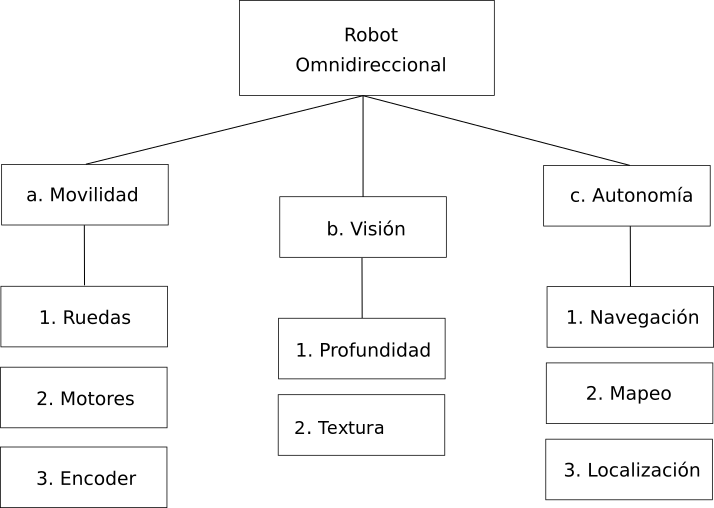
\includegraphics[scale=0.6]{imagenes/robot_omnidireccional.png}
  \label{fig:robot_omnidireccional}
  \caption{Diagrama de componentes de un robot omnidireccional. Autoría propia.}
\end{figure}


\section{Movilidad}
Existen varios aspectos a considerar cuando se diseña un robot: movilidad, control y posicionamiento. La primera hace referencia a la cantidad de movimientos que un robot puede realizar para llegar a una configuración final. Deben ser capaces de alcanzar cualquier posición y cualquier orientación en su plano de movimiento. Esto quiere decir que el marco del robot debe poseer tres coordenadas independientes del plano general de movimiento \cite{Batlle2009}.

El movimiento se puede realizar con un robot que tiene dos grados de libertad (se puede mover hacia adelante y atrás, con un ángulo de dirección), pero hay que maniobrar. Es más fácil realizar esta tarea si un robot tiene tres grados de libertad. Esto quiere decir, se puede mover hacia adelante y hacia atrás, izquierda derecha, y rotar. De esta manera, la movilidad aumenta, puesto que la cantidad de movimientos posibles que un robot puede realizar para llegar a una configuración final aumenta \cite{Batlle2009}.

Existe un tipo de ruedas, conocidas como ruedas omnidireccionales, que están compuestas de pequeños rodillos que habilitan el deslizamiento de la rueda en cierta dirección. En particular, las ruedas mecanum, como las que se muestran en la figura, 


\section{¿A quién va dirigido el trabajo escrito?}
  
Una guía útil para tomar decisiones sobre qué incluir en el trabajo escrito es tener conciencia de cuál es el público meta de la lectura. Esto marca grandes diferencias, pues, por ejemplo, para un sector externo de la carrera habría que iniciar explicando conceptos básicos; mientras que, si está dirigido a profesores, se omite casi todo tema introductorio y se enfoca en los aspectos novedosos del trabajo. Sin embargo, este último enfoque puede dejar a muchos lectores con vacíos importantes de teoría.

Tomando en consideración lo anterior, la recomendación de la Escuela es la siguiente:

\begin{quote}
Los lectores del trabajo escrito del Proyecto Eléctrico son estudiantes de ingeniería eléctrica del último año de carrera.
\end{quote}

Esta recomendación permite tomar algunas decisiones importantes, por ejemplo:

\begin{description}
\item[¿Se debe explicar el concepto de resistencia eléctrica?] No, porque se asume a todo lector familiar con el tema\footnote{A pesar de eso, la explicación de la resistencia eléctrica se ha incluido muchas veces en trabajos escritos.}. Sería justificable cuando el proyecto estudia algún concepto fundamental relacionado con la resistencia.
\end{description}

Como regla de dedo:

\section{``Antecedentes'' vs ``Marco Teórico'' vs ``Estado del Arte''}

\section{Las partes del documento escrito}

\subsection{Asuntos preliminares}

\subsubsection{Portada}

\subsubsection{Hoja de aprobación}

\subsubsection{Resumen}

\subsubsection{Resumen en inglés}

\subsubsection{Dedicatoria}

\subsubsection{Agradecimientos}

\subsubsection{Índices}

\subsection{Cuerpo del documento}

\subsubsection{Primer capítulo: introducción}

\subsubsection{Segundo capítulo: teoría}

\subsection{Contenido posterior}

\subsubsection{Apéndices}

\subsubsection{Bibliografía}

\section{Convenciones básicas de formato en español}

\begin{description}
\item[Mayúsculas en los títulos] Lleva mayúscula solamente la primera letra del título, excepto por nombres propios o siglas que por su naturaleza se escriben en mayúscula.
\end{description}

% Revisar qué hay que dejar de aquí:

\section{Más explicaciones aquí}

En el segundo capítulo del informe, debe resumirse el estudio realizado sobre \emph{estado de la técnica}, en la temática relacionada con el proyecto.  Este se puede denominar ``Antecedentes'', ``Marco de referencia'', ``Base teórica'', o ``Marco teórico''.

Por tratarse de una presentación con base en la recopilación, el análisis y la síntesis de trabajos de otros autores, la referencia adecuada a los mismos, es indispensable.  Toda copia (\emph{¡plagio!}), es inaceptable.

Para indicar las fuentes bibliográficas puede utilizarse el comando del paquete \texttt{natbib} \texttt{\textbackslash cite\{bibtexkey\}} para utilizar el formato ``Autor (año)'' o el comando \texttt{\textbackslash citep\{bibtexkey\}} para mostrarla en el formato ``(Autor, año)''.

%en el siguiente párrafo se supone que se han empleado los comandos cite o citep
Por ejemplo se obtiene: ``Según Wang (1996) la frecuencia ...'' (si se cita con \texttt{cite}), o ``... para este diseño se han utilizado modelos determinísticos (Smith, 2005) y estocásticos (Bell et. al, 2010).''  (si se citan con \texttt{citep}).  

El contenido del capítulo debe ser relevante para el proyecto y no ``material de relleno'', o incluido con el único propósito de ``engordar'' el informe.

El estado de la técnica establece el \emph{punto de partida} del estudio realizado y posiblemente también, la \emph{base de comparación} para las pruebas realizadas.

Este capítulo muestra la capacidad de análisis y síntesis del estudiante.
 
%- declaración de una sección ---------------------------------------
\section{Ecuaciones}
Las ecuaciones estarán centradas y numeradas en forma secuencial por capítulo, al margen derecho.  La referencia a ellas se hará utilizando su número.

¡Texto de ejemplo! - ``El modelo utilizado para representar al proceso, es de primer orden más tiempo muerto, dado por la función de transferencia

\begin{equation}  %inclusión de ecuaciones
	P(s) = \frac{K \me^{-Ls}}{Ts+1}, \label{ec:01}
\end{equation}

\noindent donde $K$ es la ganancia, $T$ la ...''  
%si el texto después de la ecuación no inicia un nuevo párrafo y se ha insertado una linea en blanco depues de esta, es necesario poner \noindent para que el texto siguiente no tenga sangría (formato predeterminado).

Las ecuaciones forman parte del texto, por lo que deben terminarse con el signo de puntuación requerido, una coma o un punto.

Para referirse a ellas se hace uso de la etiqueta (\texttt{label}) asignada a la ecuación usando \texttt{\textbackslash eqref\{etiqueta\}} que mostrará su número.  Por ejemplo ``El modelo \eqref{ec:01} es el más utilizado para ...''

%en el siguiente párrafo se supone que se ha utilizado \eqref{etiqueta} para referencias las ecuacioenes
El texto debe mostrar ``... sustituyendo (2.4) y (2.5) en (2.2), se obtiene ...'' y no ``... sustituyendo la ecuación (2.4) y la ecuación (2.5) en la ecuación (2.2), se obtiene...''  

¡Ejemplos de ecuaciones!

Usando \texttt{equation}:
\begin{equation}
	\tau \frac{\md T_{tc}(t)}{\md t} + T_{tc}(t) = T_{gas}(t).
\end{equation}

Ecuaciones alineadas utilizando \texttt{align}:

\begin{align}
	L_1 \frac{\md i_{L_1} (t)}{\md t} &= v(t) - R_1 i_{L_1}(t) - v_c(t), \\
	C \frac{\md v_c (t)}{\md t} &= i_L(t)- \frac{1}{R_2} v_c(t).
\end{align}

\section{Figuras y cuadros}
Las figuras y los cuadros son \emph{elementos flotantes}. Aunque se le puede ``sugerir'' a \LaTeX~ donde ubicarlos, es conveniente dejarlos ``flotar''.

\subsection{Figuras}
Las referencias a las figuras debe hacerse utilizando el número asignado a ellas.  Para esto se le asigna una etiqueta (con \texttt{label}) y luego se utiliza esta para hacer la referencia (con \texttt{ref}).  Usar en el texto el término ``figura'' y no Fig.'' o ``fig.''.

La leyenda (con \texttt{caption}) de la figura, irá en la parte inferior de la misma.  Como en forma predeterminada en la clase \texttt{eieproyecto} las figuras están centradas, no es necesario usar \texttt{centering} para hacerlo.

Por ejemplo ``Considérese el diagrama de bloques mostrado en la figura en donde el proceso controlado está dado por ...''.

No utilizar ``... en la siguiente figura ...'', emplear siempre el número correspondiente para referirse a ellas.

Cuando las figuras son muy pequeñas, se puede colocar la leyenda al lado de la misma, con el ambiente \texttt{SCfigure} del paquete \texttt{sidecap}.  Un ejemplo de esto se muestra en la figura.

Cuando un gráfico muestre varias curvas, estas deben poderse distinguir, no solamente en la pantalla de la computadora, usando diferentes colores, si no también en una impresión en blanco y negro, utilizando lineas de trazos diferentes, como se muestra en la figura.

\LaTeX~ nunca coloca las figuras y los cuadros en una página anterior a la en que son incluidas.  Los elementos flotantes los coloca en la página donde se hace referencia a ellos, o en una de las siguientes.

Además, en el texto debe hacerse referencia a todas las figuras y cuadros incluidos en el informe.  Si alguno de ellos no se menciona en el texto, es que no se requiere para entender el desarrollo presentado y por lo tanto es innecesario y se podría omitir sin que se afecte el informe.

\subsection{Cuadros}
Los cuadros son el otro elemento flotante utilizado en los informes y también es conveniente dejar que \LaTeX~ los coloque en donde considere que es más adecuado.

Los cuadros no llevarán ninguna línea divisoria vertical, solo horizontales. Una en la parte superior (\texttt{toprule}), una bajo la línea de cabecera (\texttt{midrule}) y una en la parte inferior (\texttt{bottomrule}).  Normalmente basta con estas tres líneas, pero si fuera necesaria alguna otra para una división horizontal, esta debe ser del tipo \texttt{midrule}.

Se recomienda revisar los comandos para la construcción de cuadros, incluidos en el manual de la clase \texttt{memoir} \cite{memoir2011}, o en la del paquete \texttt{booktabs} \cite{fear2005}.

La leyenda (\texttt{caption}) del cuadro se mostrará en la parte superior.  Para poder referirse al cuadro (con \texttt{ref}), se le asigna una etiqueta (con \texttt{label}).

En forma predefinida, los cuadros se mostrarán centrados horizontalmente, por lo que no es necesario hacer esa indicación. 

El cuadro \ref{tab:01} es un ejemplo de un cuadro de datos simple.

%inclusión de un cuadro con datos
\begin{table}
\caption{Parámetros de los modelos.} \label{tab:01o}
		\begin{tabular}{@{}*{4}{c}@{}}
    \toprule
    $K_p$ & $T_1$ & $T_2$ & $L$ \\
    \midrule
     1,01 & 1,50 & 0,75 & 0,12 \\
		 1,15 & 2,37 & 0,15 & 0,28 \\
		 2,25 & 5,89 & 2,15 & 1,60 \\
    \bottomrule
    \end{tabular}
\end{table}

Si la primera columna corresponde a leyendas o parámetros que identifican los datos de la línea, esta debe estar justificada a la izquierda, como se muestra en el cuadro \ref{tab:AH}, que ha sido tomada de \cite{astromhagglund2006}.

\begin{table}
\caption{Parámetros de los controladores ...} \label{tab:AH}
\begin{center}
    \begin{tabular}{@{}l*{7}{c}@{}}
    \toprule
    Controller & $K$ & $K_i$ & $K_d$ & $\beta$ & $T_i$ & $T_d$ & IAE \\
    \midrule
    PD &  1,333 & 0 & 1,333 & 1 & 0 &1 & $\infty$ \\
		PI & 0,433 & 0,192 & 0 & 0,14 & 2,25 & 0 & 6,20 \\
		PID MIGO & 1,305 & 0,758 & 1,705 & 0 & 1,72 & 1,31 & 2,25 \\
		PID $T_i=4 \ T_d$ & 1,132 & 0,356 & 0,900 & 0,9 & 3,18 & 0,80 & 2,51 \\
    \bottomrule
    \end{tabular}
\end{center}
\end{table}

Se puede especificar una cabecera para más de una columna y utilizar lineas horizontales que abarquen solo unas pocas columnas, como se muestra en el cuadro \ref{tab:muestra}.

\begin{table}
\caption{Ejemplo de otro cuadro.} \label{tab:muestra}
	\begin{tabular}{@{}l*{4}{c}@{}}
	\toprule
	& \multicolumn{2}{c}{Prueba 1} & \multicolumn{2}{c}{Prueba 2} \\
	\cmidrule(l{2pt}r{2pt}){2-3}\cmidrule(l{2pt}r{2pt}){4-5} 
	& $\Delta E=5$ V & $\Delta E = -5$ V & $\Delta E = 10$ V & $\Delta E = -10$ V \\
	\midrule
	Ganancia             &  1,06 & 0,98 & 1,12 & 0,97 \\
	Tiempo subida, s  &  5,67 & 5,89 & 6,02 & 5,74 \\
	Sobrepaso máx, \%        &  2,67 & 3,25 & 2,91 & 1,56 \\
	Error, \% &  0,25 & 0,56 & 0,97 & 0,18 \\
	\bottomrule
	\end{tabular}
\end{table}

\newpage
Cuando los cuadros son pequeños (abarcan menos de la mitad del ancho del texto), se puede colocar la leyenda a la par del cuadro, utilizando el ambiente \texttt{SCtable} del paquete \texttt{sidecap}, tal como se muestra en el cuadro \ref{tab:01}.  Compare este, con el cuadro \ref{tab:01o}.

\begin{SCtable}
\caption[Parámetros de los modelos]{Parámetros de los modelos, obtenidos a partir de las tres curvas de reacción.} \label{tab:01}
    \begin{tabular}{@{}*{4}{c}@{}}
    \toprule
    $K_p$ & $T_1$ & $T_2$ & $L$ \\
    \midrule
     1,01 & 1,50 & 0,75 & 0,12 \\
		 1,15 & 2,37 & 0,15 & 0,28 \\
		 2,25 & 5,89 & 2,15 & 1,60 \\
    \bottomrule
    \end{tabular}
\end{SCtable}

% --------------------
  \chapter{Diseño}
% --------------------
\label{C:diseño}

Para la etapa de diseño, se dividirá en tres partes.

\begin{itemize}
\item La primera, será el diseño eléctrico del carrito omnidireccional, con los componentes necesarios para funcionar.
\item La segunda es el diseño del código para el carrito omnidireccional, encargado del control de los motores y la odometría de las ruedas.
\item Por último, se hablará del diseño necesario del lado de la computadora principal, para lograr la navegación y el mapeo.
\end{itemize}

\newpage

\section{Carrito omnidireccional}
Para la primera etapa, se utilizará el esquema básico presentado en la figura \ref{F:diagrama}. Se requiere de un sistema que pueda controlar los motores, y además llevar control de la odometría de las ruedas. Además se deberá incorporar el sensor de profundidad en el carrito omnidireccional.

\begin{figure}[H]
\centering
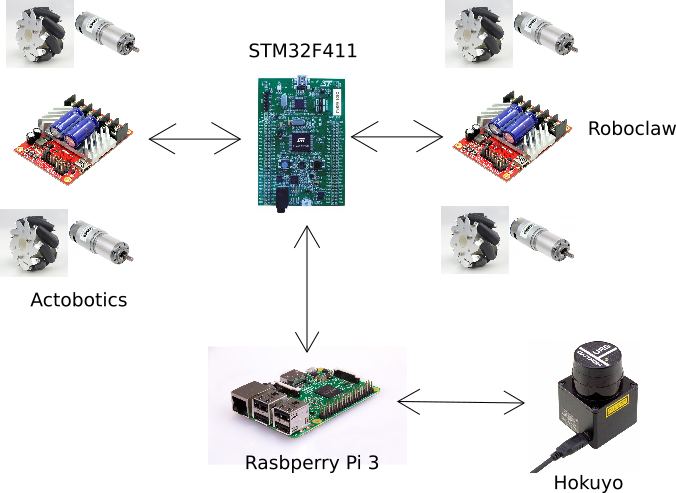
\includegraphics[scale=0.6]{imagenes/diagrama_diseno.png}
\caption{Diagrama básico de la implementación de la parte elétrica del carrito omnidireccional. Autoría propia.}
\label{F:diagrama}
\end{figure}

\subsection{Motores}

Empezando por los \textbf{motores}, se utilizarán motores DC Actobotics 638276. La hoja de fabricante con los datos en la sección de los apéndices. Además, en la tabla \ref{T:actobotics} se muestra la información más relevante de los motores a utilizar, como por ejemplo el consumo máximo, la tensión de trabajo, y la relación de los engranes.

\begin{table}[H]
\caption{Información más relevante de los motores Actobotics, a ser utilizados. Autoría propia.}
\begin{tabular}{|l|l|}
\hline
Especificación                & Valor         \\ \hline
Voltage de operación          & 6-12 VDC      \\ \hline
Corriente máxima de operación & 0.53 A        \\ \hline
Velocidad máxima sin carga    & 118 $\pm$ 12 rpm \\ \hline
Corriente máxima detenido     & 20 A          \\ \hline
Razón de los engranes         & 1/71          \\ \hline
Clicks del encoder por revolución & 3408      \\ \hline
\end{tabular}
\label{T:actobotics}
\end{table}

Se utilizarán cuatro motores, uno para cada rueda, conectados a ruedas mecanum genericas, de 6mm de diámetro. Estas son ruedas omnidireccionales con rodillos a un ángulo de $\alpha = 45^\circ$.

\subsection{Controladores}

En lo que concierne a los \textbf{controladores} de los motores, no se diseñarán, puesto que se utilizarán controladores comerciales de marca IonMotion Roboclaw. En específico, se utilizará el modelo Roboclaw 2x15A. En el cuadro \ref{T:roboclaw} se resumen los datos más importantes de este controlador.

\begin{table}[H]
\caption{Información más relevante de los controladores Roboclaw 2x15A. Autoría propia.}
\begin{tabular}{|l|l|}
\hline
Especificación                      & Valor          \\ \hline
Tensión de la batería principal     & 6-34 VDC       \\ \hline
Tensión de la batería lógica        & 6-34 VDC       \\ \hline
Bits de los contadores para encoder & 32 bits        \\ \hline
Velocidad máxima sin carga          & 118 +- 12 rpm  \\ \hline
R232 Baud Rate                      & 460,800 Bits/s \\ \hline
Tensión de I/O                      & 3.3 VDC        \\ \hline
\end{tabular}
\label{T:roboclaw}
\end{table}

Es importante mencionar, que estos controladores se utilizan para manejar los motores. Pueden manejar hasta dos motores, y son muy versátiles en cuánto a cómo se pueden utilizar. En particular, para este proyecto se usará la comunicación serial que posee el controlador. En la figura \ref{F:roboclaw} se muestran los pines que posee el roboclaw. En específico, los pines S1, y S2 se pueden utilizar como puertos USART para comunicación serial. La tabla \ref{T:pines} muestra las funcionalidades que pueden cumplir cada pin.

\begin{figure}[H]
\centering
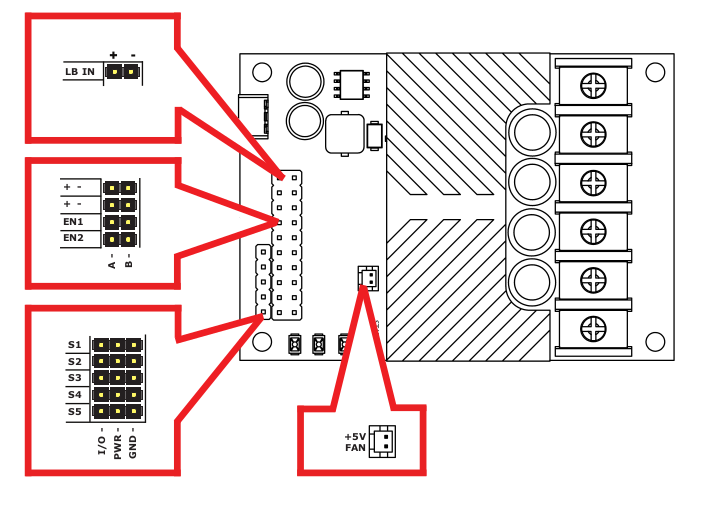
\includegraphics[scale=0.5]{imagenes/roboclaw.png}
\caption{Muestra de los pines de un Roboclaw 2x15A fabricado por IonMotion. Tomado del manual del fabricante.}
\label{F:roboclaw}
\end{figure}

\begin{table}[H]
\centering
\caption{Tabla con las funciones de los pines en un Roboclaw 2x15A fabricado por IonMotion. Tomado del manual del fabricante.}
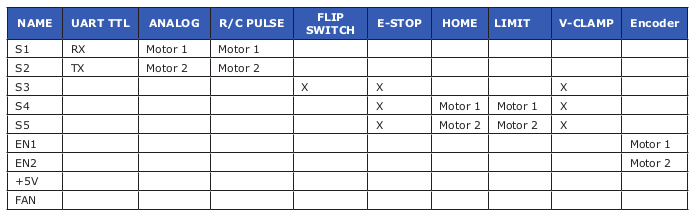
\includegraphics[scale=0.7]{imagenes/pines.png}
\label{T:pines}
\end{table}

Se utilizará una frecuencia de 115200 en la transmisión serial, ya que es la más alta soportada por el dispositivo. En el modo llamado ``Packet Serial'', el cuál funciona mediante el protocolo RS-232 para controlar la dirección y velocidad de cada uno de los motores.

El fabricante da ejemplo de código que se puede utilizar para enviar comandos, y especifica el protocola utilizado en el manual de usuario. Todas las instrucciones utilizan un checksum crc16bit para verificación de las intrucciones.

\subsection{Microcontrolador}

Siguiendo el esquema de la figura \ref{F:diagrama}, los controladores Roboclaw van conectados al \textbf{microcontrolador} STM32F411. La principal función de este microcontrolador será llevar cuenta de la odometría de cada una de las ruedas, y del robot como tal. Además, este aceptará instrucciones por USB del Raspberry Pi, de movimiento en el formato $(V_X, V_Y, W_Z)$ y enviará información de vuelta de la odometría del robot en el formato $(X_X, X_Y, \alpha_Z)$. También enviará instrucciones de movimiento a los dos controladores Roboclaw, y controlará la velocidad de cada motor por medio de un PID, en lazo cerrado con la información del encoder como entrada.

El esquema mostrado en la figura \ref{F:diagrama_stm} muestra en resumen lo que se explicó anteriormente.

\begin{figure}[H]
\centering
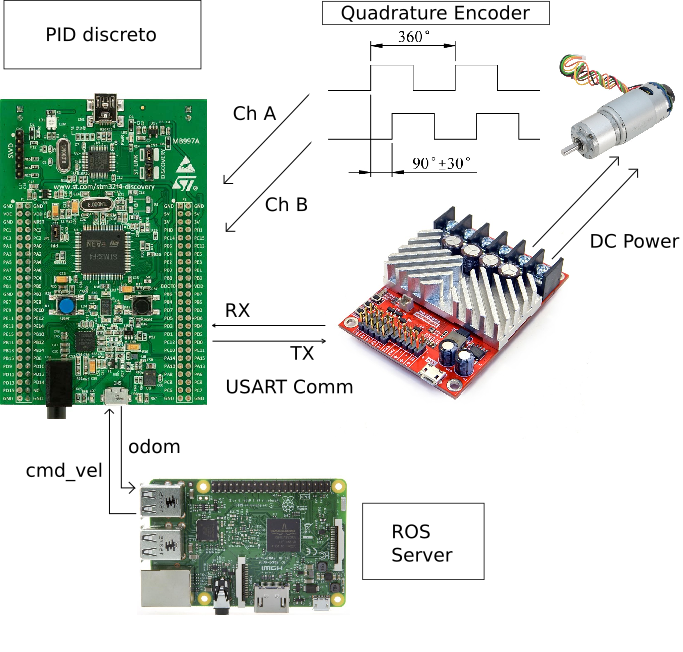
\includegraphics[scale=0.5]{imagenes/microcontrolador_diagrama.png}
\caption{Diagrama de las funciones que debe realizar el microcontrolado STM32F411. Autoría propia.}
\label{F:diagrama_stm}
\end{figure}

Es importante notar, que la programación del microcontrolador se realizará mediante las liberías libopencm3 y libopencm3-plus, las cuáles permiten escribir el código en el lenguaje de programación C. Además, el microcontrolador posee las funciones para leer los encoders directamente, puesto que posee timers que se pueden configurar en un modo para leer codificadores de cuadratura.

Información sobre el uso de encoders de cuadratura en el stm se puede encontrar en apéndice correspondiente.

\subsection{Diagrama eléctrico}

Finalmente, un diagrama de las conexiones eléctricas se puede encontrar en la figura \ref{F:conexiones}. En este diagrama se incluye la información de los pines pertinentes en cada dispositivo.

\begin{figure}[h!]
\centering
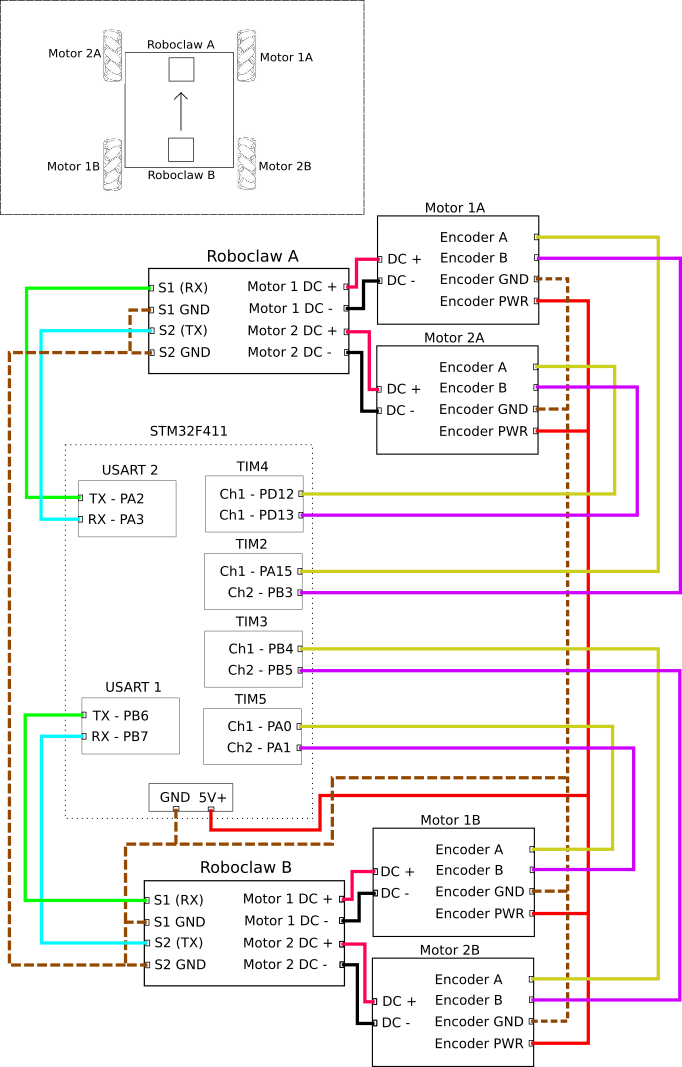
\includegraphics[scale=0.63]{imagenes/diagrama_electrico.png}
\caption{Diagrama de las conexiones eléctricas entre los dispositivos. Autoría propia.}
\label{F:conexiones}
\end{figure}

\section{Código del stm32f411}
Para el diseño del código, se debe considerar el hardware que se tiene y las funciones que este permite. A continuación se listarán las funciones que debe cumplir el código por escribir:

\begin{enumerate}
\item Librería de comunicación hacia el Roboclaw. Comandos básicos de prueba, como leer firmware, leer información de la batería, y enviar comandos de velocidad.
\item Escribir una función que sea llamada por medio de interrupciones de hardware, cada cierto tiempo constante, para llevar control de la velocidad de cada encoder, y la posición del encoder.
\item Diseñar una función que controle la velocidad de cada rueda, por medio de un control PID discreto.
\item Diseñar un protocolo de comunicación que permita recibir comandos de velocidad del Raspberry Pi, y enviar información de la odometría del robot al mismo.
\item Escribir la función que realice el cálculo de la odometría real del robot en cada interrupción por hardware.
\end{enumerate}

\subsection{Librería de comunicación}
Para escribir la librería, el manual de usuario del roboclaw menciona la estructura básica de los diferentes comandos que acepta el Roboclaw. Se implementarán un total de 6 instrucciones para proporcionar el funcionamiento básico del robot. En el apéndice se puede encontrar más información acerca de la estructura de las instrucciones. En particular nos interesan las intrucciones 0, 1, 4, 5, 21 y 24. A continuación se muestra la estructura de las instrucciones a implementar:

\begin{itemize}
\item \textbf{Instrucción 0:} Drive Forward M1. Se utiliza para mover el motor 1 hacia adelante. Tiene valores válidos desde el rango de 0 a 127, donde 127 es velocidad máxima, y 0 completamente detenido. Se manda de la siguiente manera:

Dirección, 0,  Valor, CRC(2 bytes)

\item \textbf{Instrucción 1:} Drive Backwards M1. Se utiliza para mover el motor 1 hacia atrás. Tiene valores válidos desde el rango de 0 a 127, donde 127 es velocidad máxima, y 0 completamente detenido. Se manda de la siguiente manera:

Dirección, 1, Valor, CRC(2 bytes)

Recibe lo siguiente:

0xFF

\item \textbf{Instrucción 4:} Drive Forward M2. Se utiliza para mover el motor 2 hacia adelante. Tiene valores válidos desde el rango de 0 a 127, donde 127 es velocidad máxima, y 0 completamente detenido. Se manda de la siguiente manera:

Dirección, 4,  Valor, CRC(2 bytes)

Recibe lo siguiente:

0xFF

\item \textbf{Instrucción 5:} Drive Backwards M2. Se utiliza para mover el motor 2 hacia atrás. Tiene valores válidos desde el rango de 0 a 127, donde 127 es velocidad máxima, y 0 completamente detenido. Se manda de la siguiente manera:

Dirección, 5, Valor, CRC(2 bytes)

Recibe lo siguiente:

0xFF

\item \textbf{Instrucción 21:} Read Firmware Version. Se utiliza para leer la información de la versión de software que actualmente se encuentra corriente en el controlador. Lo que se envía es bastante sencillo:

Dirección, 21

Recibe algo similar a lo siguiente:

“RoboClaw 10.2A v4.1.11”,10,0, CRC(2 bytes)

\item \textbf{Instrucción 24:} Read Logic Battery Voltage Level. Se utiliza para medir la tensión entre las terminales B+ y B-. La información se encuentra en decenas de voltage, ejemplo: 300 = 30V. A continuación se muestra lo que se debe enviar:

Dirección, 24

Recibe lo siguiente

Valor (2 bytes), CRC (2 bytes)

\end{itemize}

Esta librería se programará en el microcontrolador STM32, para poder enviar mensajes hacia el controlador de los motores. Es importante destacar que el microcontrolador posee soporte para puertos USART. Inclusive, la librería libopencm3 posee un paquete para transimisión a través de estos puertos. Sencillamente se utilizan dos comandos importantes, los cuáles son \textit{usart\_send\_blocking} y \textit{usart\_recv\_blocking}.

Respectivamente mandan y reciben un byte de información a la vez, y los bits de inicio y fin son configurables, al igual que la velocidad de transferencia, la cuál debe coincidir con la velocidad del controlador Roboclaw. Además de estos, existen otros parámetros que se deben configurar para el funcionamiento correcto del puerto de comunicación. La figura \ref{F:usart} muestra un ejemplo de cómo configurar un puerto usart utilzando la librería libopencm3.

\begin{figure}[H]
\centering
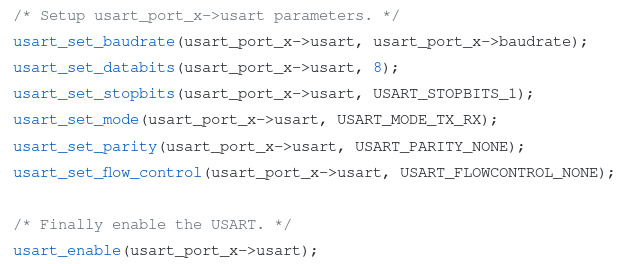
\includegraphics[scale=0.5]{imagenes/usart.png}
\caption{Ejemplo de configuración de un puerto USART utilizando la librería libopencm3. Autoría propia.}
\label{F:usart}
\end{figure}

\subsection{Encoder}

Para llevar el conteo de la cantidad de ticks que ha ocasionado un encoder en un timer del stm32f411, se debe leer constantemente el estado de cada timer, y transferir la información a una variable donde se lleve la cuenta de los ticks. Esta lectura debe de ser en intervalos de tiempo constante, para a su vez poder calcular la velocidad del motor.

El microcontrolador stm32f411 posee una función llamada systick, el cuál es un contador que produce una bandera cuando llega al valor de recarga, el cuál puede ser configurado. Esta bandera es utilizada para llamar una subrutina, que ha de ser ejecutada en el momento en que se produce la bandera.

Por lo tanto, se obtienen interrupciones en intervalos contantes, que son producidas cada cierta cantidad de ciclos de reloj. La figura \ref{F:systick} muestra un ejemplo de cómo inicializar el contador. La variable llamada SYS\_TICK\_AUTORELOAD tiene unidades en ciclos.

\begin{figure}[H]
\centering
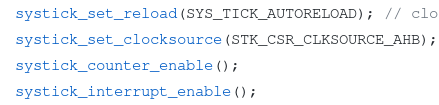
\includegraphics[scale=0.5]{imagenes/systick.png}
\caption{Ejemplo de inicialización del systick utilizando la librería libopencm3. Autoría propia.}
\label{F:systick}
\end{figure}

En la interrupción, se debería de actualizar una variable que lleve control de los ticks que han sucedido desde el inicio del programa. Además, se deberá revisar una bandera que se activa cuando el timer respectivo al encoder llega a 0.

La bandera relacionada a este evento se llama TIM\_SR\_UIF en el contexto de la librería libopencm3. En particular, de la mencionada librería se deberán utilizar tres comandos importantes, los cuáles son:

\begin{itemize}
\item \textbf{timer\_get\_counter(TIMER\_PERIPHERAL):} Esta función retorna el valor del contador, el cuál es un entero sin signo de máximo 32 bits.

\item \textbf{timer\_get\_flag(TIMER\_PERIPHERAL, FLAG):} Esta función se utiliza para obtener el valor de una bandera específica del timer. Retorna un valor booleano.

\item \textbf{timer\_clear\_flag(TIMER\_PERIPHERAL, FLAG):} Limpia el valor de la bandera, por lo tanto la pone en Falso. No retorna nada.
\end{itemize}

\subsection{Control PID}

Al igual que en el caso anterior, esta función de control del pid debe ser llamada en intervalos de tiempo constante, para que la acción del controlador siempre tenga la misma rapidez. Por lo tanto es prudente incorporar esta función como parte de la subrutina systick.

La figura \ref{F:pid_diagrama} muestra el PID en cuestión a programar. La función debe comprobar si existe una diferencia entre la velocidad actual y la deseada, y dado el error producido por la resta de ambas, multiplicar este valor por una constante Kp. Utilizando la suma del error además, multiplicar eso por una constante Ki. Finalmente, el cambio del error, será multiplicado por una constante Kd. La suma de los tres componentes, da como resultado la acción a mandar al controlador.

\begin{figure}[H]
\centering
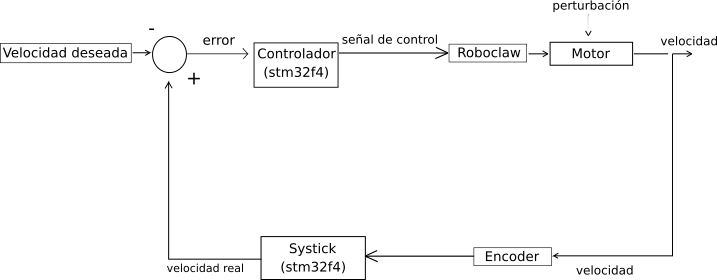
\includegraphics[scale=0.7]{imagenes/diagrama_pid.png}
\caption{Diagrama del PID a programar utilizado para controlar la velocidad de cada motor. Autoría propia.}
\label{F:pid_diagrama}
\end{figure}

Los valores de Kp, Ki, y Kd deben ser fácilmente ajustables desde el ciclo principal, para su ajuste correspondiente. Algo a notar, diferente de un PID convencional, es que la acción del controlador tiene un límite, puesto que el controlador de los motores no acepta señales análogas. Esto quiere decir que se debe manejar la condición en donde la señal de control sea mayor al número 127 (que es la máxima señal de control que acepta el Roboclaw).

\subsection{Protocolo de comunicación USB}

\label{libreria}

Para esta función, será necesario utilizar la librería llamada libopencm3-plus, la cuál contiene funciones que permiten utilizar comandos básicos como putc y getc en el buffer del puerto USB que trae el microcontrolador stm32f411.

El protocolo de comunicación deberá ser binario, para mayor eficiencia en la transmisión. Al igual que en el caso del protocolo de comunicación hacia el roboclaw, se utilizará una verificación crc16 para todas las instrucciones. Se diseñarán varias instrucciones con el fin de enviar comandos de velocidad desde la pc principal, y además poder recibir información de la odometría actual del robot.

A continuación se listan las instrucciones por implementar, y la estructura de cada una:

\begin{itemize}
\item \textbf{Move Robot:} Esta instrucción recibe comandos de velocidad en $x$, $y$, y rotación en $z$. Se recibe lo siguiente:

m (1 byte ascii), $V_X$ (float 32 bits), $V_Y$ (float 32 bits), $\omega_Z$ (float 32 bits), 10, 0, CRC (2 bytes)

Se envía de vuelta el checksum calculado localmente:

CRC (2 bytes)

\item \textbf{Read Odometry:} Esta instrucción envía de vuelta la información de la odometría actual del robot. Se recibe lo siguiente:

o (1 byte ascii), 10, 0, CRC (2 bytes)

Se envía de vuelta lo siguiente:

$X_X$ (float 32 bits), $X_Y$ (float 32 bits), $\theta_Z$ (float 32 bits), CRC (2 bytes)

\item \textbf{Read Velocity:} Esta instrucción envía de vuelta la velocidad actual del robot. Se recibe lo siguiente:

v (1 byte ascii), 10, 0, CRC (2 bytes)

Se envía de vuelta lo siguiente:

$V_X$ (float 32 bits), $V_Y$ (float 32 bits), $\omega_Z$ (float 32 bits), CRC (2 bytes)

\item \textbf{Reset Robot:} Esta instrucción devolverá el robot a estado estacionario, y regresará la odometría del robot a 0,0,0. Se recibe lo siguiente:

r (1 byte ascii), 10, 0, CRC (2 bytes)

Se envía de vuelta lo siguiente:

CRC (2 bytes)
\end{itemize}


Las instrucciones anteriores son las únicas necesarias para lograr el correcto funcionamiento de la navegación. Sin embargo, se escribirán las siguientes instrucciones adicionales para revisar que no existan errores.

\begin{itemize}
\item \textbf{Read Wheel Velocities:} Envía de vuelta las velocidades de cada una de las ruedas. Se recibe lo siguiente:

e (1 byte ascii), 10, 0, CRC (2 bytes)

Se envía de vuelta lo siguiente:

$V_{1A}$ (float 32 bits), $V_{2A}$ (float 32 bits), $V_{1B}$ (float 32 bits), $V_{2B}$ (float 32 bits), CRC (2 bytes)

\item \textbf{Read Serial Comm failures:} Envía la cantidad de fallos de la comunicación entre el stm32f411 y el roboclaw desde el último reset robot. Se recibe lo siguiente:

t (1 byte ascii), 10, 0, CRC (2 bytes)

Se envía de vuelta lo siguiente:

Fallos (float 32 bits), CRC (2 bytes)

\item \textbf{Read Wheel Position:} Envía la posición de las ruedas desde el último reset robot en cantidad de ticks. Se recibe lo siguiente:

h (1 byte ascii), 10, 0, CRC (2 bytes)

Se envía de vuelta lo siguiente:

$X_{1A}$ (float 32 bits), $X_{2A}$ (float 32 bits), $X_{1B}$ (float 32 bits), $X_{2B}$ (float 32 bits), CRC (2 bytes)

\end{itemize}

\subsection{Odometría Real del robot}

Para realizar el cálculo de la odometría real del robot, se utilizarán las ecuaciones descritas en la nota teórica. Para esto, se utiliza la velocidad angular de cada una de las ruedas en un instante dado, se calcula el cambio en la posición de cada rueda en un instante dado, y con esto obtenemos el cambio en la posición del robot en ese instante. Finalmente, estos cambios se suman constantemente en variables globales, para mantener la posición global del robot. A continuación, el diagrama mostrado en \ref{F:calculo_odoemtría} muestra el diagrama de flujo de lo anteriormente mencionado.

\begin{figure}[H]
\centering
\includesvg[width=450pt]{diagramas/diagrama_odometry}
%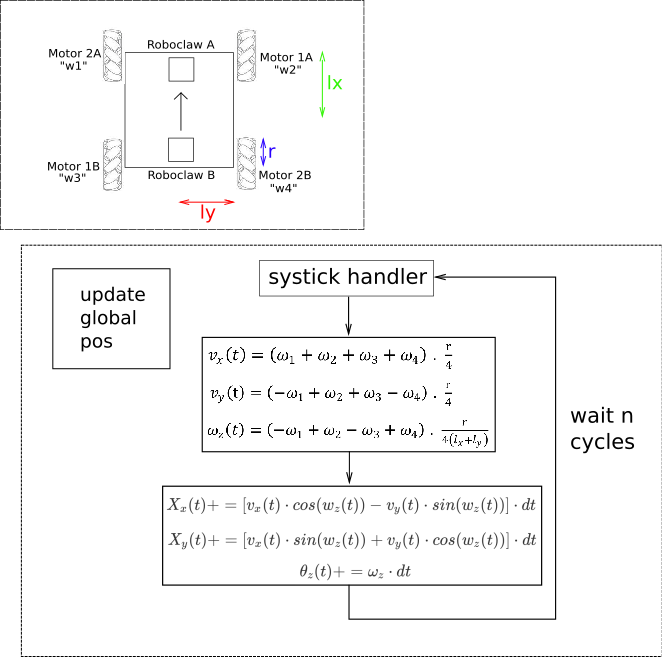
\includegraphics[scale=0.7]{imagenes/diagrama_globalpos.png}
\caption{Diagrama de la actualización de la posición global. Autoría propia.}
\label{F:calculo_odometria}
\end{figure}

Es importante mencionar que para la escritura del código, se utilizará la plataforma GitHub. El código mencionado anteriormente se puede encontrar en el repositorio \textbf{arcoslab/stm32-roboclaw}.

\subsection{Diagrama completo del código}
A continuación en la figura \ref{F:main} se muestra un diagrama completo que muestra un poco de pseudo-código.

\begin{figure}[H]
\centering
%\includesvg[width=450pt]{diagramas/diagrama_codigoprincipal}
%\includesvg[scale=1]{diagramas/diagrama_codigoprincipal}
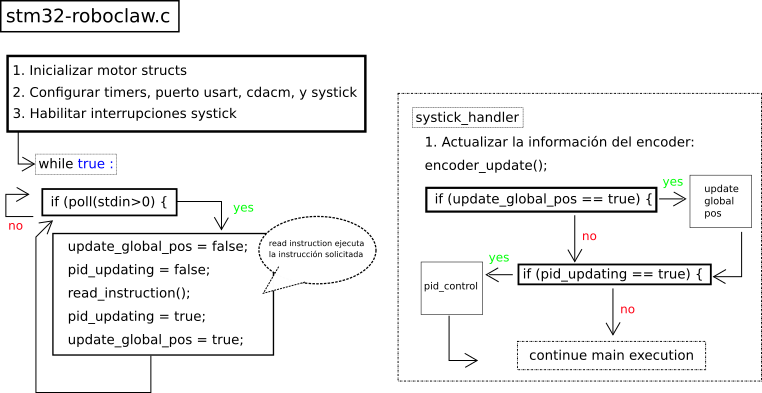
\includegraphics[scale=0.8]{imagenes/diagrama_main.png}
\caption{Esquema de lo que contiene el archivo principal del programa a correr en el microcontrolador. Autoría propia.}
\label{F:main}
\end{figure}

\newpage

\section{Código de la computadora principal}

En la computadora principal se correrá el servidor de ROS que interconectará el robot omnidireccional con el stack de navegación. Hay varios requisitos que se deben cumplir para que el stack de navegación funcione correctamente. La figura \ref{F:navigation_stack} muestra un diagrama de la interacción entre Navigation Stack y el robot deseado. Los cuadros que se encuentran de color azulado, son específicas de la plataforma.

\begin{figure}[H]
\centering
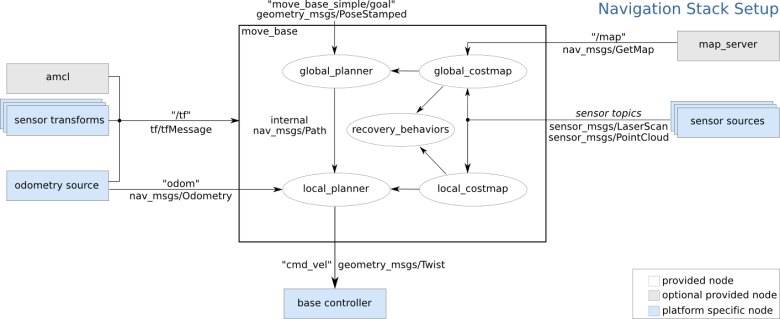
\includegraphics[scale=0.7]{imagenes/overview_tf_small.png}
\caption{Revisión de configuración para el stack de navegación. Tomado de ROS.}
\label{F:navigation_stack}
\end{figure}

Es necesario por lo tanto, crear un nodo en ros que posea las siguientes características:

\begin{enumerate}
\item Publicación de la información de los sensores láser en el tópico LaserScan para sensores de profundidad 2D, o PointCloud para sensores en 3D.
\item Publicación de la odometría actual del robot en el tópico llamado ``odom''. Esta es la información de la posición de la base con respecto al mundo.
\item Publicación del árbol de transformación en el tópico ``tf''.
\item Subscripción al nodo ``cmd\_vel'', para recibir instrucciones de movimiento de la base.
\end{enumerate}

\subsection{Sensores láser}

Se tienen dos tipos de sensores que se utilizarán a lo largo del desarrollo de este proyecto, los cuáles son un Kinect V2 y un sensor Hokuyo. Ambos tienen soporte en ROS, por lo que en esta sección, el trabajo a realizar es instalar el software que ya existe.

\begin{itemize}
\item Para el caso del sensor Kinect V2 se utilizó el software que se encuentra en el repositorio \href{https://github.com/code-iai/iai_kinect2}{Iai\_Kinect2}. En este repositorio se encuentran una serie de herramientas para calibrar, realizar el registro de la información de profundidad, y utilizar libfreenect2 por debajo. Esta librería utiliza aceleración gráfica con OpenCL, por lo que es importante tener los mejores drivers de la tarjeta de video disponible.

\item Para el uso del sensor Hokuyo, también existe un paquete llamado \href{https://github.com/ros-drivers/hokuyo_node}{Hokuyo\_node} que puede ser utilizado para la lectura del sensor directamente al tópico LaserScan.
\end{itemize}

La salida de ambos sensores puede ser visualizada en \href{http://wiki.ros.org/rviz}{Rviz}, un visualizador del ambiente de ROS.

\subsection{Odometría}

\label{seccionodometria}

La información de la odometría del robot se puede leer directamente del mismo, sin embargo la librería del lado de la computadora principal debe ser implementada primero. Los comandos son los mismos que los explicados en la sección del \hyperref[libreria]{Protocolo de comunicación USB}, sin embargo lo que se envía y recibe está inverso. Se implementará esta ``driver'' en Python, por su facilidad y modularidad.

La figura \ref{F:odometria_python} explica la relación necesaria entre el nodo principal, y este driver para obtener la información de odometría.

ROS posee una librería llamada \textbf{rospy} la cuál es útil para realizar nodos de ros que puedan publicar mensajes. En particular, los mensajes de odometría se pueden publicar utilizando un tipo de mensaje llamado \textbf{Odometry}, el cuál se encuentra en la librería \textbf{nav\_msgs.msg}.

Los mensajes de este tipo poseen las características que se encuentran resumidas en el cuadro \ref{T:odometría}.

\begin{table}[H]
\caption{Contenido de un mensaje del tipo ``Odometry'' en el entorno ROS. Autoría propia.}
\begin{tabular}{|l|l|}
\hline
Tipo de mensaje en el contenido    & Nombre           \\ \hline
std\_msgs/Header                   & header           \\ \hline
string                             & child\_frame\_id \\ \hline
geometry\_msgs/PoseWithCovariance  & pose             \\ \hline
geometry\_msgs/TwistWithCovariance & twist            \\ \hline
\end{tabular}
\label{T:odometría}
\end{table}

El mensage del tipo PoseWithCovariance contiene la información de la posición actual, mientras que el TwistWithCovariance contiene la información de la velocidad actual del robot.

\subsection{Árbol de Tf}

La mayoría de paquetes en Ros requieren que un árbol de transformaciones sea publicado utilizando la librería Tf. Esta librería se utiliza para definir las compensaciones necesarias para cada objeto del mundo cuando se da un movimiento.

\begin{figure}[H]
\centering
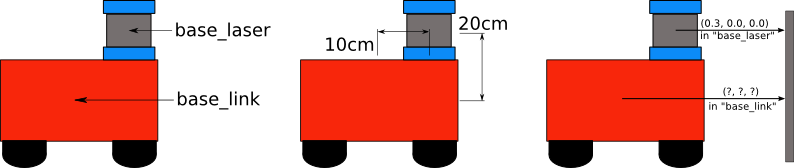
\includegraphics[scale=0.6]{imagenes/simple_robot.png}
\caption{Ejemplo de la utilidad de Tf. Tomado de \cite{ROSTF}.}
\label{F:tf}
\end{figure}

La figura \ref{F:tf} muestra un robot omnidireccional, que tiene un láser encima de él. Cada vez que el robot se mueve, deberíamos de ajustar la posición actual del láser, puesto que ahora el láser no está en la misma posición que antes. Este ajuste se podría hacer manualmente cada vez que se actualiza la posición del robot, sin embargo cuando se tienen muchos objetos en el mundo que dependen de la posición actual del robot, estas transformaciones se vuelven engorrosas. Por lo tanto, es más sencillo utilizar tf, y establecer la relación que existe entre la base y el sensor láser \cite{ROSTF}.

Hay varias formas de establecer esta relación. Sin embargo, la más sencilla cuando se tiene una relación estática (no cambia con el tiempo) es definir la misma en el launch file utilizado para levantar el nodo de ROS. La figura \ref{F:launchfile} muestra un ejemplo de cómo realizar esta transformación.

\begin{figure}[H]
\centering
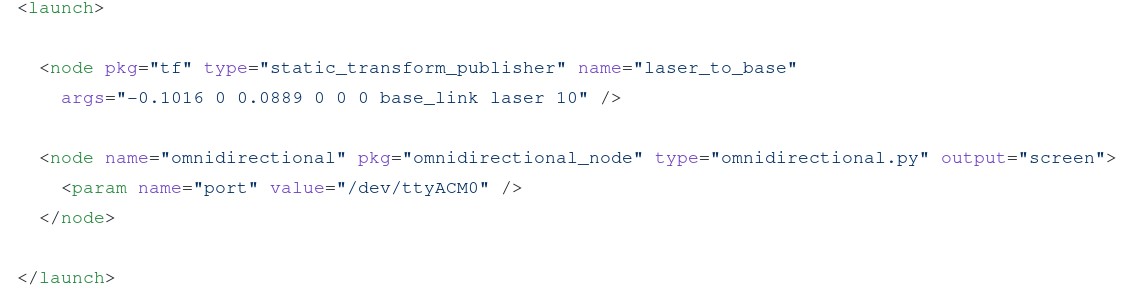
\includegraphics[scale=0.4]{imagenes/launch_file.png}
\caption{Ejemplo de un launch file en ROS que habilita un árbol tf. Autoría propia.}
\label{F:launchfile}
\end{figure}

\subsection{Comandos de velocidad de la base}

Al igual que con la sección de \hyperref[seccionodometria]{Odometría}, en este nodo es necesario un intermediario que pueda comunicarse con el stm32f411 y mande la instrucción correspondiente para comandar la velocidad. Un diagrama que explica la relación se puede encontrar en la figura \ref{F:rosnode}.

\begin{figure}[H]
\centering
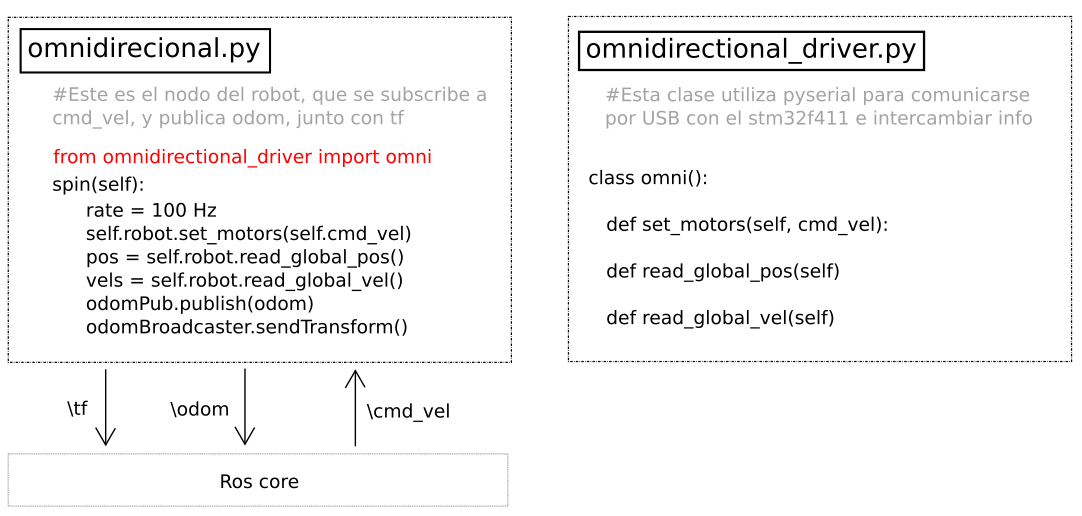
\includegraphics[scale=0.4]{imagenes/diagrama_rosnode.png}
\caption{Diagrama de las interacciones entre el nodo de ROS y el driver de la conexión USB. Autoría propia.}
\label{F:rosnode}
\end{figure}


%% --------------------------------
  \chapter{Sobre el uso de \LaTeX}
% --------------------------------
\label{C:sobre_LaTeX}

\section{Introducción}

\LaTeX~ es un editor de texto bajo el paradigma de edición de texto ``lo que ve es lo que quiere decir'' (WYSIWYM, del inglés \emph{What You See Is What You Mean}) en el que se utiliza un lenguaje de descripción de formato\footnote{En ese sentido parecido al HTML}. Este paradigma es diferente a su contraparte y tradicional paradigma WYSIWYG (del inglés \emph{What You See Is What You Get}, ``lo que ve es lo que obtiene''), en el que se edita el texto y los demás elementos en una interfaz gráfica. Este es el caso de herramientas de ofimática como Microsoft Office, OpenOffice y LibreOffice y editores gráficos de todo tipo.

\begin{quote}
\LaTeX~ ``...es un sistema de composición lógica, por oposición a los sistemas de composición visual o programas WYSIWYG (\ldots) Con el sistema \LaTeX, lo que el autor escribe y ve en la pantalla del ordenador es el contenido del documento y su estructura lógica, pero entre estos y el documento compuesto hay un paso intermedio de procesamiento o \emph{compilación} del documento mediante el sistema \LaTeX'' \cite{Valiente2001}.
\end{quote}

Existe bibliografía extensa (incluyendo \cite{Valiente2001}\cite{Gratzer2001}\cite{Krishnan2003}\cite{Oetiker2014}\cite{Wikibooks2016}) donde se puede ampliar sobre \LaTeX. Así mismo, en Internet hay gran cantidad de tutoriales, comunidades y foros sobre el tema, como en \cite{StackExchange2016}. Se recomienda consultar estas fuentes para ampliar las posibilidades de escritura con este lenguaje.

En este capítulo se incluyen y explican algunos de los elementos básicos y más utilizados para la redacción en \LaTeX: ecuaciones, figuras, tablas, además de referencias a bibliografías, secciones, entre otras cosas, y puede ser utilizado como base para la elaboración del trabajo escrito del curso.

\subsection{¿Por qué \LaTeX? (opcional)}

\LaTeX~ es un paradigma de edición de texto utilizado ampliamente en la comunidad científica y tecnológica de todo el mundo, en publicaciones, revistas, libros y más. 

Tiene la virtud de facilitar la composición de un documento bien diseñado que ahorra toda la cuestión de forma para el editor.

La siguiente lista\footnote{Adaptado de \url{http://haptonstahl.org/latex/whyuse.php}} explica algunos puntos acerca del uso de \LaTeX.

\begin{description}

\item[Documentos estructurados] 
Es más fácil crear documentos estructurados en \LaTeX~ que en Word u otros editores. Un documento estructurado es un \emph{paper}, artículo, libro o tesis con capítulos, secciones, subsecciones, apéndices, tablas de contenidos, índices, etc. Los capítulos y secciones usualmente son enumerados secuencialmente, están listados en una tabla de contenidos, etc. Cuando se hacen cambios, todas las referencias relativas tienen que ser actualizadas. Todo esto es trivialmente fácil en \LaTeX.

Si no se quiere pensar acerca del formato y solo se quiere que el \emph{software} haga las cosas verse bien, hay que usar \LaTeX.

\item[Ecuaciones] 
Es más fácil y rápido escribir símbolos matemáticos utilizando \LaTeX~ que con MS Word. Una o dos páginas de fórmulas probablamente harán caer MS Word. Cientos de páginas de fórmulas no harán caer a \LaTeX.

\item[Calidad de tipografía e impresión] 
La escritura en \LaTeX~ es superior a la de otros procesadores de texto. Más referencias sobre esto en \url{http://nitens.org/taraborelli/latex}.

\end{description}

%%%%%%%%%%%%%%%%%%%%%%%%%%%%%%%%%%%%%%%%%%%%%%
\section{Las partes de un documento de \LaTeX}
%%%%%%%%%%%%%%%%%%%%%%%%%%%%%%%%%%%%%%%%%%%%%%

\subsection{Preámbulo y cuerpo del documento}
%%%%%%%%%%%%%%%%%%%%%%%%%%%%%%%%%%%%%%%%%%%%%

Los archivos \texttt{.tex} de donde se generan los documentos en \LaTeX~ tienen dos grandes secciones: el encabezado o preámbulo y el cuerpo del documento.

En el \textbf{encabezado} del documento se definen los parámetros más importantes del documento, y se invocan los ``paquetes'' que permiten la edición de características especiales. Entre las características que se pueden definir aquí están: tamaño del papel, tamaño y tipo de tipografía, tipo de documento (reporte, artículo, libro, carta\ldots), numeración, autor, fecha, título y más. 

Además de estas definiciones generales, se deben cargar todos los \textbf{paquetes} que permiten hacer ediciones especiales como: introducir hipervínculos, agregar colores, agregar imágenes, editar encabezados y pies de página, etc. 

Para utilizar un paquete se escribe la instrucción \verb+\usepackage[opciones]{nombredelpaquete}+, donde las opciones están definidas por cada paquete particular. 

Por ejemplo \verb+\usepackage[spanish]{babel}+. El paquete Babel permite cambiar la lengua del documento (en inglés por defecto), y entre paréntesis cuadrado se especifica que sea español.

Los paquetes que utiliza \LaTeX~ están en un repositorio (ver Sección \ref{S:programas}). La documentación de los paquetes puede encontrarse en la página de CTAN (\textit{Comprehensive TEX Archive Network}), \url{https://www.ctan.org/}.

Uno de los elementos más importantes de \LaTeX~ es el \emph{entorno}. Un entorno (\emph{environment}) siempre inicia con \verb+\begin{nombredelentorno}+ y finaliza con \verb+\end{nombredelentorno}+. Dentro de él, todo el contenido va a tener un formato característico dependiendo del tipo de entorno. Las ecuaciones, figuras y tablas tienen su propio entorno. Hay otros para listas numeradas, resumen, teoremas, texto centrado\ y más. El mismo cuerpo del documento es un gran entorno \texttt{document}.

A continuación se describirá el uso de algunos de los entornos más importantes: ecuaciones, tablas y figuras.

\subsection{Ecuaciones}
%%%%%%%%%%%%%%%%%%%%%%%

Hay tres tipos de ecuaciones posibles: unas en línea, o dentro del párrafo, otras en modo \emph{display} con numeración y sin numeración. 

\begin{description}

\item [Las ecuaciones en línea] están rodeadas por los símbolos \verb+$ $+ (una forma abreviada de crear el entorno). Se utilizan cuando se coloca una fórmula en un párrafo, por ejemplo $ {{B}_{f}}\ge 0,2 $, que no lleva numeración y que debe estar alineada con el texto. \LaTeX~ se encargará de ajustar su tamaño y ubicación, como cuando se introduce una raíz cuadrada $ \sqrt {{b^2} - 4ac} $ o una integral  $ \int_0^\infty e^{-x}\,\mathrm{d}x $. 

\item [Las ecuaciones numeradas] se hacen dentro del entorno \texttt{equation}. Ejemplos de ecuaciones se muestran a continuación.

\begin{verbatim}
\begin{equation}
x_{1,2} = \frac{-b \pm \sqrt{b^2 - 4ac}}{2a}
\end{equation}
\end{verbatim}

\begin{equation}
x_{1,2} = \frac{-b \pm \sqrt{b^2 - 4ac}}{2a}
\end{equation}

\begin{equation}\label{E:desigualdad}
{B}_{f}\ge 0,2
\end{equation}

\begin{equation}\label{E:anchodebanda}
BW\ge 500\text{ MHz}
\end{equation}

donde $ {B}_{f} $ es el ancho de banda fraccional y se define como:

\begin{equation}\label{E:fraccional}
{{B}_{f}}=\frac{BW}{{{f}_{c}}}=\frac{\left( {{f}_{H}}-{{f}_{L}} \right)}{{\left( {{f}_{H}}+{{f}_{L}} \right)}/{2}\;}
\end{equation}

donde $f_H$ y $f_L$ son las frecuencias superior e inferior de la banda de transmisión de -10 dB, $ BW $ es el ancho de banda y $f_c$ la frecuencia central.

El estilo de la numeración depende del tipo de documento (\texttt{article}, \texttt{report}, \texttt{book}\ldots) y obedecerá (si no se especifica lo contrario) la secuencia numérica.

\item [La ecuaciones no numeradas] se deben utilizar en ocasiones, sobre todo cuando se trata de pasos intermedios o cálculos y no la deducción de alguna expresión. Para ello se deben utilizar los símbolos \verb+\[+ y \verb+\]+ (otra forma abreviada de crear el entorno) para rodear la ecuación.

\[
 \lim_{x \to \infty} \exp(-x) = 0
\]

\[
 R_{pu} = 2,7~\si{\kilo\ohm}
\]

\end{description}

Será necesario también en ocasiones incluir texto dentro de las ecuaciones. Pero es necesario escribir este texto dentro de los comandos \verb+\text{}+, \verb+\textbf{}+ o similares, para que se les aplique el espaciado y formato correctos. De otro modo sucede lo que se muestra en la ecuación (\ref{E:sintexto}), mientras que la ecuación (\ref{E:contexto}) muestra el uso corregido, incluyendo cierto formato añadido para resaltar.

\begin{equation}\label{E:sintexto}
Ciclo de trabajo = \frac{Tiempo en alto}{Per\acute{i}odo}
\end{equation}

\begin{equation}\label{E:contexto}
\text{Ciclo de trabajo} = \frac{\textsf{Tiempo en alto}}{\textbf{Per\'{i}odo}}
\end{equation}

A pesar de que la escritura de ecuaciones directamente en \LaTeX~ puede resultar algo complicada al principio, basta con una rápida investigación en la vasta información de las referencias suministradas y en la red\footnote{Hay muchas comunidades de usuarios en internet en foros y demás que resuelven estos problemas típicos} para encontrar la forma de realizar la ecuación deseada. Como alternativa, se puede utilizar un editor gráfico de ecuaciones como \href{http://www.dessci.com/en/products/mathtype/}{MathType} y de ahí exportar a \LaTeX\footnote{Para hacerlo: en la ventana de edición de ecuaciones de MathType se debe ir a \textsf{Preferences / Cut and Copy Preferences}, en la ventana emergente se debe seleccionar la opción \textsf{MathML or TeX} y en la lista desplegable escoger \textsf{LaTeX 2.09 and later}. En la misma ventana de edición se selecciona y copia la ecuación. La barra de estado mostrará: \textsf{Translated (LaTeX 2.09 and later)}.}. Es necesario, aún así, aprender los comandos básicos que facilitan y hacen más rápida la composición de fórmulas.

También se pueden editar ecuaciones en la aplicación en internet disponible en \url{http://rinconmatematico.com/latexrender/} en la cual se puede ver el resultado de la ecuación editada.

\subsection{Figuras}\label{S:Figuras}
%%%%%%%%%%%%%%%%%%%%%%%%%%%%%%%%%%%%%

Para las figuras existe un entorno llamado \verb+figure+, dentro del cual se ubican y configuran las imágenes.

Para ``llamar'' al archivo se debe hacer una referencia a su ubicación. Si está ubicada en la misma carpeta del documento se escribe \verb+nombre_de_la_imagen.jpg+\footnote{O cualquier formato de imágenes soportado, como .png, .gif y otros}. Pero los archivos de imágenes, de preferencia y por una cuestión de orden, deben colocarse dentro de una carpeta dedicada. Entonces, si está dentro de una carpeta se indica \verb+./carpeta/nombre_de_la_imagen.jpg+. Para subir un nivel en las carpetas se utiliza \verb+../carpeta/subcarpeta/nombre_de_la_imagen.jpg+. 

La imagen ``Nube de tormenta con rayos y lluvia'' es un ejemplo de imagen insertada.

\begin{figure}[H]
\centering
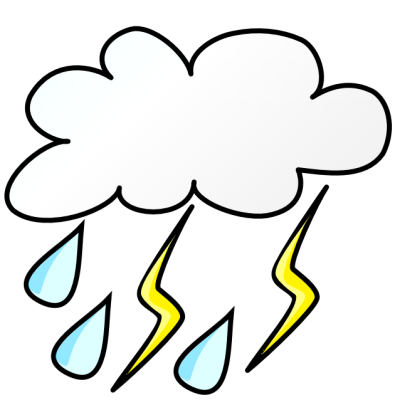
\includegraphics[width=0.2\textwidth]{./imagenes/tormenta.png} 
\caption{Nube de tormenta con rayos y lluvia}
\label{F:tormenta}
\end{figure}

La instrucción para insertar la gráfica es:


\begin{lstlisting}[]
\begin{figure}[H]
\centering
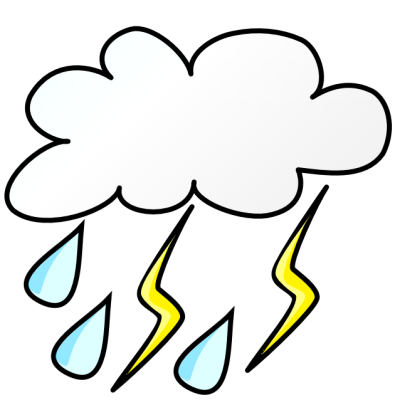
\includegraphics[width=0.2\textwidth]{./imagenes/tormenta.png} 
\caption{Nube de tormenta con rayos y lluvia}
\label{F:tormenta}
\end{figure}
\end{lstlisting}

La descripción es la siguiente:

\begin{itemize}\itemsep0pt \parskip0pt \parsep0pt
\item \verb+\begin{figure}[H]+ en la línea 1 inicia el entorno de la figura y declara que será ubicada inmediatamente luego del texto, con \verb+[H]+.
\item \verb+\centering+ en la línea 2 es una instrucción abreviada para indicar que la figura estará centrada.
\item \verb+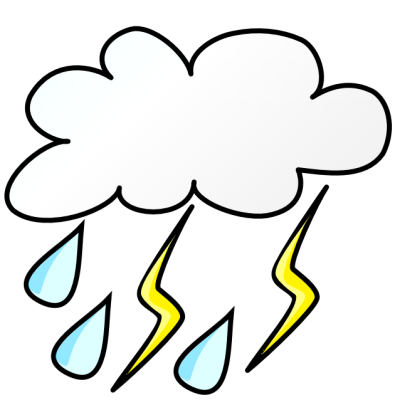
\includegraphics[width=0.2\textwidth]{./imagenes/tormenta.png}+ es la instrucción para insertar el archivo de la imagen, junto con indicaciones adicionales sobre el tamaño (un 20 \% del ancho del texto).
\item \verb+\caption{Nube de tormenta con rayos y lluvia}+ la instrucción  \texttt{caption}\footnote{En inglés, es bastante explícita esta instrucción, y en general puede decirse lo mismo de todos los comandos de \LaTeX, (ver por ejemplo \textsf{footnote}, \textsf{includegraphics}, \textsf{subsection}, etc.)} es el pie de figura con el nombre y la explicación. El número de figura lo inserta \LaTeX~ automáticamente.
\item \verb+\label{F:tormenta}+ es una etiqueta para referencia dentro de otras partes del texto.
\item \verb+\end{figure}+ cierra el entorno de la figura.
\end{itemize}

Como buena práctica, se recomienda nombrar el archivo de la imagen igual que la etiqueta, y con \textit{un nombre representativo}. Los nombres no deben tener espacios ni tildes ni eñes. Por ejemplo: \verb+senal_entrada_sinusoidal.jpg+.

\LaTeX, por defecto, va a ubicar las imágenes arriba o debajo de la página, y no inmediatamente después del texto en el que se escribe dentro del código, excepto que se indique lo contrario con \verb+\begin{figure}[h!]+ o con \verb+\begin{table}[H]+ utilizando el paquete \verb+float+.

Adicionalmente, se puede ubicar varias imágenes dentro de un mismo entorno de figura, como en la Figura \ref{F:subfiguras}. Ahí se muestran cuatro figuras distintas dentro del mismo entorno, donde se puede hacer referencia al transistor en \ref{F:subfig1}, al LED en \ref{F:subfig2}, al fotoconductor en \ref{F:subfig3} y al circuito integrado en \ref{F:subfig4}.

\begin{figure}[h!]
\centering
\subfloat[Transistor (texto que aparece en el índice)][Transistor en encapsulado TO-220]{
	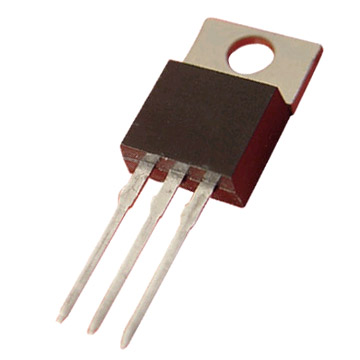
\includegraphics[width=0.2\textwidth]{./imagenes/transistor.jpg}
	\label{F:subfig1}}
\qquad
\subfloat[LED][LED blanco de baja potencia]{
	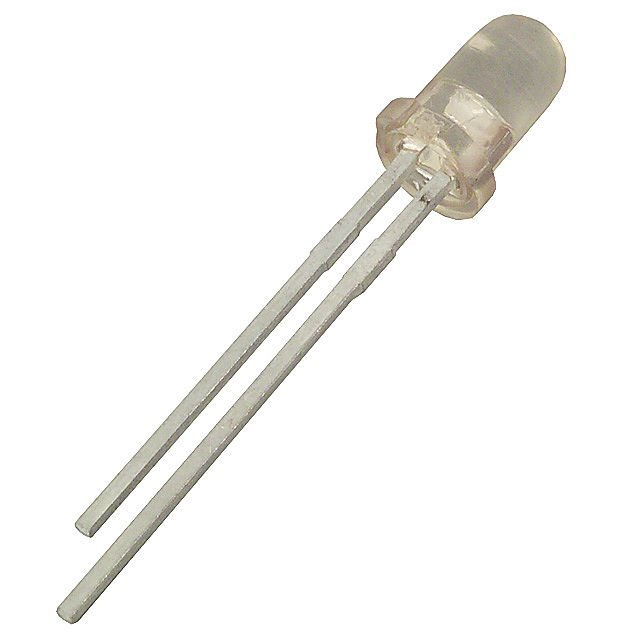
\includegraphics[width=0.2\textwidth]{./imagenes/led.jpg}
	\label{F:subfig2}}
\\
\subfloat[Fotoconductor][Fotoconductor]{
	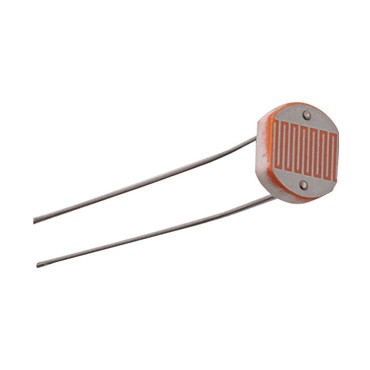
\includegraphics[width=0.2\textwidth]{./imagenes/fotoconductor.jpg}
	\label{F:subfig3}}
\qquad
\subfloat[Circuito integrado][Circuito integrado en encapsulado DIP-8]{
	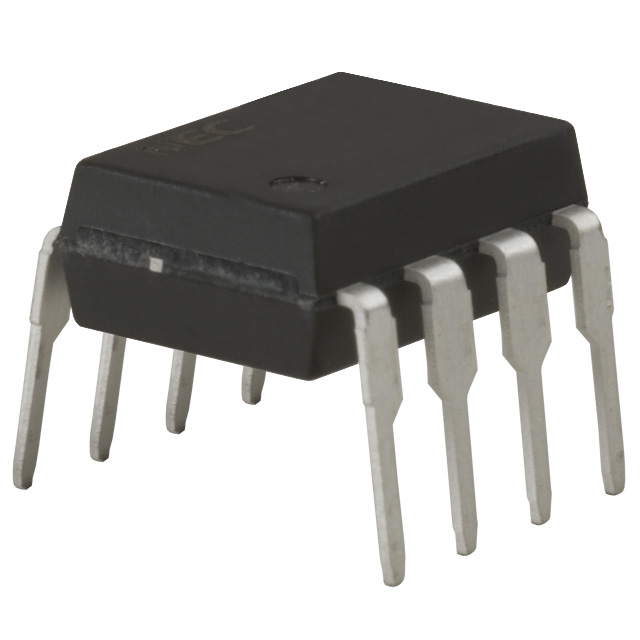
\includegraphics[width=0.2\textwidth]{./imagenes/integrado.jpg}
	\label{F:subfig4}}
\caption{Una figura con varias subfiguras, utilizando el paquete \texttt{subfig}}
\label{F:subfiguras}
\end{figure}

\subsection{Tablas}
%%%%%%%%%%%%%%%%%%%

Para las tablas se debe utilizar el entorno \verb+table+.

Aquí hay dos casos posibles:

\begin{description}

\item [Que la tabla debe construirse en \LaTeX] y en ese caso se debe usar el entorno \verb+tabular+, que a su vez se incluye dentro de \verb+table+.

\item [Que la tabla es en realidad una imagen] si fue generada por otro programa o fue escaneada, etc. Esta imagen entonces se incluye dentro del entorno \verb+table+ para que sea tratada como tal (y se numere como tabla, y se incluya en el índice de tablas, y se hagan las referencias como tablas, etc.).

\end{description}

Como ejemplo sencillo, la Tabla \ref{T:ejemplo} muestra una tabla con líneas verticales, declaradas como \verb+c | c+, que significa \textit{centrado - línea vertical - centrado}, y líneas horizontales, declaradas como \verb+\hline+ después de cada línea salto de línea (\verb+\\+).

\begin{table}
\caption{Comparación de velocidad de UWB con otros estándares alámbricos e inalámbricos}
\label{T:ejemplo}
\begin{center}
\begin{tabular}{ c | c}
\hline
\textbf{Velocidad [Mbits/s]} & \textbf{Estándar} \\ 
\hline
480 & UWB, USB 2.0 \\ 
200 & UWB (4 m) \\
110 & UWB (10 m) \\ 
90 & Fast Ethernet \\ 
54 & 802.11a \\ 
20 & 802.11g \\ 
11 & 802.11b \\ 
10 & Ethernet \\ 
3 & Bluetooth \\ 
0,256 & ZigBee \\ 
\hline
\end{tabular}
\end{center}
\end{table}

La instrucción \verb+\begin{tabular}{ | c | c |}+ genera un cuadro con líneas verticales en ambos lados, como en la Tabla \ref{T:ejemploconlineas}. 

Cuando se tiene un documento de dos o más columnas, es importante notar que una tabla puede ser muy grande y no quepa en una sola columna, por tanto debe especificarse que se acomode a todo lo ancho de la página. Esto es sencillo: basta con escribir \verb+table*+ al inicio y al final cuando se declara el entorno en \verb+\begin{} ... \end{}+.

\begin{table*}
\caption[Título en el índice]{Título que aparece en el pie de figura o encabezado de la tabla. Puede ser bastante amplio y explicar con más detalle. Debido a que el título que aparece en el índice es corto, no hay problema de que se exceda el espacio apropiado ahí.}
\label{T:ejemploconlineas}
\begin{center}
\begin{tabular}{| c | c |}
\hline
\textbf{Velocidad [Mbits/s]} & \textbf{Estándar} \\ 
\hline
480 & UWB, USB 2.0 \\ 
200 & UWB (4 m), 1394a (4,5 m) \\
110 & UWB (10 m) \\ 
90 & Fast Ethernet \\ 
54 & 802.11a \\ 
20 & 802.11g \\ 
11 & 802.11b \\ 
10 & Ethernet \\ 
3 & Bluetooth \\ 
0,256 & ZigBee \\ 
\hline
\end{tabular}
\end{center}
\end{table*}

Del mismo modo que en las figuras, \LaTeX~ por defecto colocará la tabla en la parte superior de la siguiente página, excepto que se indique lo contrario (con \verb+\begin{table}[h!]+)\footnote{Para mejor manejo de la posición de figuras, tablas y otros, utilizar el paquete \textsf{float}}.

\begin{table}
\caption{Otra tabla utilizando el paquete \texttt{booktabs}}
\label{T:otratabla}
\centering
\begin{tabular}{c l r r}
\toprule
\multicolumn{2}{c}{Producto} \\
\cmidrule(r){1-2}
Cantidad & Descripción & Precio unitario & Precio total  \\
\midrule
3  & Transistores 	& 250	& 750	\\
4  & Osciladores   	& 500   & 2000 \\
3  & Amp Ops     	& 600   & 1800	\\
10 & Resistores  	& 25    & 250	\\
10 & Capacitores	& 50 	& 500	\\
\midrule 
\multicolumn{3}{r}{TOTAL} & \textbf{5300} \\
\bottomrule
\end{tabular}
\end{table}

%%%%%%%%%%%%%%%%%%%%%%%%%%%%%
\section{Herramientas útiles}
%%%%%%%%%%%%%%%%%%%%%%%%%%%%%

%----------------------------------
\subsection{Referencias a figuras, tablas, ecuaciones, secciones y otros}

Es fundamental a lo largo del texto hacer referencias a figuras, tablas, ecuaciones, secciones y otros. Todos estos elementos tienen una etiqueta \verb+\label{}+ asociada a cada uno. 

La instrucción para hacer la referencia a esta etiqueta es \verb+\ref{}+.

Así entonces, se puede hacer referencia a las ecuaciones (\ref{E:desigualdad}), (\ref{E:anchodebanda}) y (\ref{E:fraccional}), a la Figura \ref{F:tormenta} y a la Tabla \ref{T:ejemplo} desde cualquier parte del texto, sin importar la numeración, que será asignada automáticamente por \LaTeX.

Es buena práctica nombrar las ecuaciones como \verb+\label{E:ecuacion}+, las tablas como \verb+\label{T:tabla}+, las figuras como \verb+\label{F:figura}+, y así sucesivamente, es decir, con una E, T, F o S antepuestas para identificar de qué se trata en cada caso, y con un nombre representativo. 

No es bueno hacer referencias relativas como ``la siguiente figura'' o ``la tabla anterior'' porque en realidad no se sabe la ubicación final dentro del texto. Hay que notar que tanto las tablas como las figuras, a menos de que se especifique lo contrario\footnote{Como se ha explicado, una forma de cambiar esto es colocando [h!] o [H] (de \emph{here}) junto al inicio del entorno.}, se colocarán al principio o al final de la página, en donde el programa lo considere mejor por motivo de espacio. Es mejor una referencia absoluta tal como figura \ref{F:tormenta} o ecuación (\ref{E:fraccional}). 

En editores de escritorio, algunas veces es necesario compilar dos o tres veces para que se carguen correctamente los números de referencia.

\subsection{Citas bibliográficas}
%%%%%%%%%%%%%%%%%%%%%%%%%%%%%%%%%

Los trabajos académicos requieren de referencias a las fuentes de información, invariablemente. Es necesario entonces considerar cómo crear una bibliografía y cómo referirse a las fuentes dentro del texto. 

Se puede hacer una bibliografía ``a mano'', en el que se le da la edición necesaria a cada entrada\footnote{En el código fuente de este documento hay un ejemplo de bibliografía tipo ``plain''.}. Sin embargo, BibTeX es una mejor alternativa, que permite administrar y modificar fácilmente una gran cantidad de entradas, además de que hace posible la reutilización de las referencias, en otros documentos.

\subsubsection{BibTeX}

\href{http://www.bibtex.org/}{BibTeX} es un programa de manejo de referencias. En este documento se utiliza de la siguiente forma:

\begin{itemize}
\item En un archivo llamado \texttt{bibliografia.bib} se introducen todas las referencias utilizadas, con el formato especial para ello. Ejemplo:
\begin{verbatim}
@BOOK {Valiente2001,
    author    = "Valiente Feruglio, G.",
    title     = "Composición de Textos Científicos con LaTeX",
    publisher = "Alfaomega",
    year      = "2001",
    address   = "México D.F.",
    edition   = "primera"
}
\end{verbatim}
Una buena herramienta para editar estas entradas se encuentra en \url{http://truben.no/latex/bibtex/}, sin embargo, considerar los sistemas de manejo bibliográfico de la siguiente sección.

\item Dentro del texto se hace referencia a las fuentes. La instrucción para hacer una cita es \verb+\cite{+\textit{clave}\verb+}+, dentro del cual se coloca la etiqueta, clave o \textit{key} asignada a la bibliografía (el primer espacio en la entrada de BibTeX de ejemplo), usualmente el apellido del primer autor y el año de publicación, por ejemplo: \verb+\cite{Valiente2001}+, que resulta en \cite{Valiente2001}.

\item Finalmente, al final del trabajo, se colocan las instrucciones 
\begin{verbatim}
\bibliographystyle{estilo}
\bibliography{nombrearchivo.bib}
\end{verbatim}
donde \texttt{estilo} es uno de los varios formatos posibles para las citas y las referencias (ver una lista en \url{https://www.sharelatex.com/learn/Bibtex_bibliography_styles}), y la segunda instrucción se encarga de colocar el título, y todas las entradas \textbf{que han sido citadas}, en el orden y el formato necesarios. Ahí es donde la ventaja de BibTeX se hace más evidente. 

\item En programas de edición de escritorio (Texmaker,\ldots) es necesario compilar varias veces y en una secuencia específica para que se genere la bibliografía. Esta secuencia es: \texttt{latex} \textgreater~ \texttt{bibtex} \textgreater~ \texttt{latex} \textgreater~ \texttt{latex}. En las plataformas de edición en línea (Overleaf,\ldots) esto se hace automáticamente.
\end{itemize}

\subsubsection{Sistemas de manejo bibliográfico}

En trabajos de investigación es necesario recurrir a muchas referencias (en tesis y otros, fácilmente más de 50) y el manejo de estas se puede tornar engorroso. Actualmente, varias plataformas ofrecen un manejo automatizado y muy conveniente de referencias. A continuación se presentan algunas opciones.

\begin{multicols}{2}
\begin{description}
\item[Mendeley] \url{http://www.mendeley.com/}
\item[Readcube] \url{http://www.readcube.com/}
\item[Docear] \url{http://www.docear.org/}
\item[Citavi] \url{http://www.citavi.com/}
\item[EndNote] \url{http://endnote.com/}
\item[JabRef] \url{http://jabref.sourceforge.net/}
\end{description}
\end{multicols}

\subsection{Formato}
%%%%%%%%%%%%%%%%%%%%

%---------------------------------------
\subsubsection{Cambiar el tipo de letra}

La tipografía de \LaTeX~ por defecto es la \href{https://en.wikipedia.org/wiki/Computer_Modern}{Computer Modern}. Es fácil de identificar y ampliamente utilizada (por la popularidad de \LaTeX) en muchas publicaciones científicas.

Esta plantilla de Proyecto Eléctrico utiliza la tipografía \href{http://www.linuxlibertine.org/}{Libertine}. 

Es útil, sin embargo, cambiar de tipografía en todo el documento o en algunas secciones\footnote{¡Cuidado! Demasiada libertad para cambiar el formato del documento puede derivar en malas decisiones de diseño gráfico. Ejemplo usual: utilizar Comic Sans (no disponible aquí).}.

Una referencia de la mayoría de tipografías disponibles para \LaTeX~ se encuentra en \url{http://www.tug.dk/FontCatalogue/}. Por ejemplo, la siguiente instrucción en el preámbulo convierte todo el texto a DejaVu Sans.

\begin{verbatim}
\usepackage{DejaVuSans}
\renewcommand*\familydefault{\sfdefault} 
\usepackage[T1]{fontenc}
\end{verbatim}

La instrucción \verb+{\fontfamily{qag}\selectfont ...texto...}+ genera {\fontfamily{qag}\selectfont un texto en otra tipografía. Para restringir la selección, el texto debe estar rodeado por llaves}. El código \texttt{qag} representa el tipo de letra. Una lista de tipos de letras y sus códigos, junto con más opciones se puede encontrar \href{https://www.sharelatex.com/learn/Font_typefaces}{aquí} y \href{http://tex.stackexchange.com/questions/25249/how-do-i-use-a-particular-font-for-a-small-section-of-text-in-my-document}{aquí}.

%-----------------------
\subsubsection{Unidades}

Las unidades deben escribirse separadas de la magnitud. Cuando se hace en una ecuación se presenta el problema que muestra la ecuación (\ref{E:sinunidades}). Para resolver este problema hay que incluir algún paquete que permita introducir unidades correctamente. En este documento se eligió \verb+siunitx+. La ecuación (\ref{E:conunidades}) muestra el uso corregido de las unidades en las ecuaciones. Del mismo modo, se puede poner de ejemplo: $C_s = \SI{0.1}{\micro\farad}$, $T_c = \SI{27}{\degreeCelsius}$. 

\begin{equation}\label{E:sinunidades}
{V}_{i}\ge 1,3 mV
\end{equation}

\begin{equation}\label{E:conunidades}
{V}_{i} \ge 1,3~\si{\milli\volt}
\end{equation}

O también el siguiente ejemplo:

\begin{equation}\label{E:unidades}
V = I_L \times R_L = \left( 0,25~\si{\milli\ampere} \right) \times \left( \SI{4}{\kilo\ohm} \right) = 1~\si{\volt} 
\end{equation}

%--------------------------------------------
\subsubsection{Otras herramientas de formato}

\begin{enumerate}
\item Las notas de pie\footnote{Que se insertan escribiendo la instrucción inmediatamente después del texto a comentar, como en este caso.}, utilizando la instrucción \verb+\footnote{}+.
\item Las comillas, que colocan con estos símbolos ``especiales'' y no las comillas del teclado. 
\item La palabra \LaTeX~ se escribe con el comando \verb+\LaTeX+. Debe escribirse el símbolo \verb+~+ después de la instrucción para que genere un espacio adecuado entre palabras, de otro modo \LaTeX queda pegado.
\item Las \textbf{negritas} se escriben con el comando \verb+\textbf{}+ (de \textit{\textbf{b}old \textbf{f}ace})
\item Las \textit{cursivas} se escriben con el comando \verb+\textit{}+ (de \textit{\textbf{it}alics})
\item Las \textsc{versales} se escriben con el comando \verb+\textsc{}+ (de \textit{\textbf{s}mall \textbf{c}aps})
\item Las \texttt{monoespacio} se escriben con el comando \verb+\texttt{}+ (de \textit{\textbf{t}ele\textbf{t}ype})
\item El comando \verb+\emph{}+ se utiliza para \emph{resaltar} un texto, muy similar a \verb+\textit{}+, con la diferencia que \textit{el resaltado depende del \emph{contexto} del párrafo}.
\item Hay varios tamaños de guiones: -, -- (con \verb+--+) y --- (con \verb+---+).
\item Se puede especificar la fecha de hoy, \today, utilizando el comando \verb+\today+.
\item El paquete \verb+hyperref+ permite la inclusión de hipervínculos, tanto a lugares externos del documento como internos (observe las referencias a tablas, figuras o ecuaciones o las citas bibliográficas). También incorpora los   marcadores que se muestran en los lectores de pdf y que se utilizan para navegación del documento. Por ejemplo, se puede hacer referencia a la Sección \ref{S:Figuras} donde se explica la inclusión de figuras (y hacer clic al hipervínculo y seguirlo).
\item Las listas numeradas (como esta) se hacen con el entorno \verb+\begin{enumerate}+, las listas con viñetas utilizando \verb+\begin{itemize}+.
\item Se pueden crear comandos especiales para insertar textos o símbolos definidos por el usuario. La instrucción es \verb+\newcommand{\comando}{Texto a introducir}+.
\item Por ejemplo, si no se quiere escribir cada vez ``Escuela de Ingeniería Eléctrica'' y además se le quiere dar un formato especial, entonces se puede indicar en el preámbulo 

\verb+\newcommand{\EIEx}{\textsc{Escuela \Lightning~ Ingeniería Eléctrica}}+ 

y así se crea el comando \verb+\EIEx+ que genera: \EIEx.
\item[--] Se puede utilizar un guión (o cualquier símbolo) en lugar de la numeración o las viñetas en una lista, con la instrucción \verb+[-]+ al lado de \verb+\item+.
\item[\Biohazard] Ejemplo de símbolo como viñeta\footnote{Las instrucciones \texttt{Lightning} y \texttt{Biohazard} son parte del paquete de símbolos especiales \texttt{marvosym}.}.
\end{enumerate}

\subsection{Figuras con PGF/Ti\textit{k}Z}
%%%%%%%%%%%%%%%%%%%%%%%%%%%%%%%%%%%%%%%%%%

PGF/Ti\textit{k}Z es un conjunto de lenguajes para producir gráficos vectoriales a partir de una descripción geométrica y algebraica\footnote{Tomado de su descripción en Wikipedia.}. Tiene grandes capacidades y una documentación exhaustiva.

La Figura \ref{F:tikz} es un ejemplo relativamente sencillo de las capacidades de Ti\textit{k}Z.

\begin{figure}[H]
\centering
	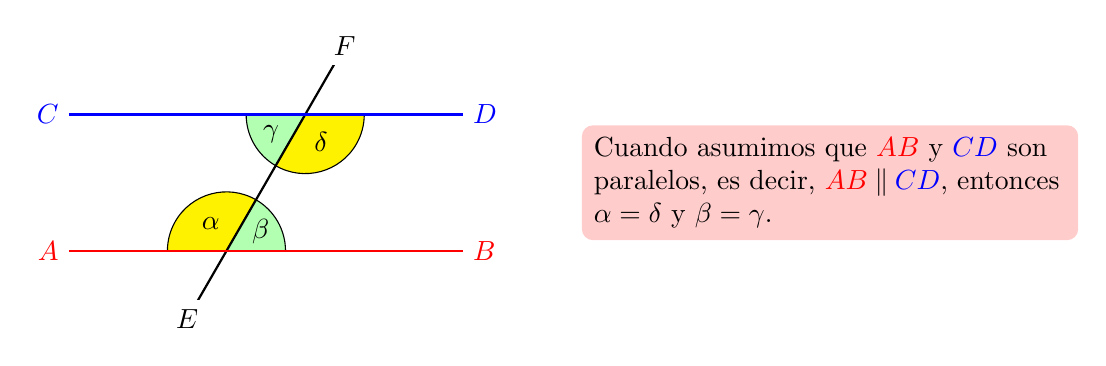
\begin{tikzpicture}
	  \draw[fill=yellow] (0,0) -- (60:.75cm) arc (60:180:.75cm);
	  \draw(120:0.4cm) node {$\alpha$};
	  \draw[fill=green!30] (0,0) -- (right:.75cm) arc (0:60:.75cm);
	  \draw(30:0.5cm) node {$\beta$};
	  \begin{scope}[shift={(60:2cm)}]
	    \draw[fill=green!30] (0,0) -- (180:.75cm) arc (180:240:.75cm);
	    \draw (30:-0.5cm) node {$\gamma$};
	    \draw[fill=yellow] (0,0) -- (240:.75cm) arc (240:360:.75cm);
	    \draw (-60:0.4cm) node {$\delta$};
	  \end{scope}
	  \begin{scope}[thick]
	    \draw  (60:-1cm) node[fill=white] {$E$} -- (60:3cm) node[fill=white] {$F$};
	    \draw[red]                   (-2,0) node[left] {$A$} -- (3,0) node[right]{$B$};
	    \draw[blue,shift={(60:2cm)}] (-3,0) node[left] {$C$} -- (2,0) node[right]{$D$};
	    \draw[shift={(60:1cm)},xshift=4cm]
	    node [right,text width=6cm,rounded corners,fill=red!20,inner sep=1ex]
	    {
	      Cuando asumimos que $\color{red}AB$ y $\color{blue}CD$ son paralelos, es decir, ${\color{red}AB} \mathbin{\|} \color{blue}CD$, entonces $\alpha = \delta$ y $\beta = \gamma$.
	    };
	  \end{scope}
	\end{tikzpicture}
\caption[Ejemplo de uso de PGF/Ti\textit{k}Z]{Ejemplo de uso de PGF/Ti\textit{k}Z, pero solo una muestra de sus capacidades.}
\label{F:tikz}
\end{figure}

Una buena cantidad de ejemplos están disponibles en \url{http://www.texample.net/tikz/} y la documentación (incluyendo un manual de uso de más de 700 páginas) está en \url{https://www.ctan.org/pkg/pgf?lang=en}.

%---------------------------------------
\subsection{Gráfico de datos y funciones con \texttt{pgfplots}}

%---------------------------------------
\subsection{Circuitos con Circuitikz}

El paquete \texttt{circuitikz} permite la creación de circuitos eléctricos y electrónicos. La Figura \ref{F:ampop} es un ejemplo.

\begin{figure}
  	\centering
		 \begin{circuitikz}[american]
		  \draw
		  % El amplificador operacional
		  (0,0) node[op amp] (opamp) {} node[] {{\tiny Amp Op}}
		  
		  % Las entradas
		  (opamp.-) node[circ] {} to[R, l_=$R_1$] ++(-2,0) node[ocirc] {} node[left] {$V_{s}$}
		  (opamp.+) -- ++(0,-0.5) node[ground] {} 
		  
		  % El lazo de realimentación
		  (opamp.-) -- ++(0,1)  to[R, l=$R_2$] ++(2,0) -| (opamp.out) {}
		  
		  % La salida
		  (opamp.out) -- ++(0.5,0) node[circ] {} to[R, l=$R_L$] ++(0,-2) to [short, i_=$I_o$] ++(0,0) node[ground] {}
		  (opamp.out) -- ++(1,0) node[ocirc] {} node[right]{$V_o$}
		  
		  ;
		\end{circuitikz}
    \caption[Amplificador inversor]{Amplificador inversor con un amplificador operacional cuya relación entrada--salida está dada por $V_o = -\frac{R_2}{R_1} V_s$.}
    \label{F:ampop}
\end{figure}

\begin{figure}
\centering
\begin{circuitikz}
\draw
	(0,0)
    	to [V, l=50~\si{\volt}] (0,2) to (0,3)
        to [R, l=$20~\si{\kilo\ohm}$] (5,3) to (5,2)
        to [vR, l=$R$] (5,0)
        to (0,0)
  	(0,2)
    	to [R, l_=$5~\si{\kilo\ohm}$] (5,2)     
;
\end{circuitikz}
\caption{Circuito básico.}
\label{F:circuitobasico}
\end{figure}

\begin{figure}
\centering
\begin{circuitikz}
\draw
	(0,0) node[ground]{}
    	to [V, l=(``Arenal'') $V_{1}$] (0,3)
        to [short] (0.5,3) node[circ]{}
   	(5.5,3)
        to [short] (5.5,4)
        to [R, l=$R_{1}$, i<=$I_{1}$] (3,4)
        to [cV, l=$v_{1}$] (0.5,4)
        to [short] (0.5,3)   
   	(6,3)
    	to [short] (5.5,3)
        to [short] (5.5,2)
        to [R, l=$R_{3}$, i<=$I_{2}$] (3,2)
        to [cV, l=$v_{3}$] (0.5,2)
        to [short] (0.5,3)
	(6,3) node[circ]{}
    	to [generic, i_=$I_{L}$, v^=$v_{L}$] (6,0) node[ground]{}
   	(6,3)
    	to [R, l=$R_{2}$, i<=$I_{3}$] (8.5,3)
        to [cV, l=$v_{2}$] (11,3)
    (11,0) node[ground]{}
        to [V, l_=$V_{2}$ (``Miravalles'')] (11,3)
;
\end{circuitikz}
\caption[Circuito de transmisión de potencia]{Circuito de transmisión de potencia por varias líneas conductoras desde centros de generación y con sistemas de ajuste de la corriente.}
\label{F:transmisionpotencia}
\end{figure}

\begin{figure}
\centering
\begin{circuitikz}
\draw 
(0,0)	to [battery, l_=$V_i$] (0,3)
		to [R, l_=$R_1$] (2.5,3)
        to [cV, l_=$A v_x$] (5,3)
        to [short] (6,3)
        to [vR, l_=$R_T$, i=$i_{R_T}$] (6,0) node[ground]{}
        to [short] (0,0)
(6,3)	to [short] (7,3)
(6,0)	to [short] (7,0)

;
\draw (2.5,3) to [open, v=$v_x$] (2.5,0);
\draw (2.5,3) node[circ]{};
\draw (2.5,0) node[circ]{};

\draw[dashed] (-0.8,-0.8) rectangle (4.8,3.8);
\draw (-0.8,-0.8) node [above right]{Fuente de corriente};

\draw (7,-0.5) rectangle (9,3.5);
\draw (8,1.5) node [align=center]{Circuito \\ de acople};

\draw 
(9,3)	to [short] (10,3)
		to [R, l_=$R_2$] (12,3)
		to [generic, l_=$Y$, v^=$v_Y$] (14,3)
(9,0)   to [short] (14,0) node[ground]{}
		to [cV, l=$A v_z$] (14,3)
(14,0)	to [short] (15.3,0)
		to [open, v>=$v_o$] (15.3,3)
		to [short] (14,3)
;
\draw (12,3)	to [open, v=$v_z$] (12,0);
\draw (12,3) node[circ]{};
\draw (12,0) node[circ]{};

\draw[dashed] (9.8,-0.8) rectangle (14.8,3.8);
\draw (9.8,-0.8) node [above right]{Amplificador};

\draw (15.3,3) node[circ]{} node[right]{$a$};
\draw (15.3,0) node[circ]{} node[right]{$b$};
\end{circuitikz}
\caption[Circuito de acondicionamiento y amplificación]{Circuito de acondicionamiento y amplificación de la señal de un sensor resistivo $R_T$, dependiente de la temperatura.}
\label{F:acondicionamiento}
\end{figure}

\begin{figure}
\centering
\begin{circuitikz}

% PNP Q1
\draw
	(0,4) 	node[pnp,rotate=90](Q1){} node[above]{$Q_1$}
;
% NPN Q2
\draw
	(0,1.5) 	node[npn,rotate=180,yscale=-1](Q2){} node[left]{$Q_2$}
;
% Op Amp
\draw
	(3,1.5) 	node[op amp,rotate=180,yscale=-1](CMP){} node[]{AMP}
;
% Resistores
\draw
	(6,4) node[circ]{} 
    	to [R, l=$R_1$] (6,2) 
    	to [R, l=$R_2$] (6,0) node[ground]{}
;
% Conectores
\draw
	(-1.5,4) 	node[ocirc]{} node[above]{$V_{IN}$} 
    		to [short] (Q1.emitter)
  	(Q1.base) to [short] (Q2.collector)
    (Q2.emitter) to [short] (0,0) node[ground]{}
    (CMP.out) to [short] (Q2.base)
    (Q1.collector) to [short] (7,4) node[ocirc]{} node[above]{$V_{OUT}$}
    (CMP.-) to [short] (6,2) node[circ]{}
    (4.5,0) node[ground]{} to [battery,l_=$V_{R}$] (4.5,1) to [short] (CMP.+) 
;
\end{circuitikz}
\caption{Regulador lineal de tensión con lazo de control.}
\label{F:reguladorlineal}
\end{figure}

\begin{figure}
\centering
\begin{circuitikz} 
\draw
	(0,0) node[op amp,yscale=-1] (opamp) {}
    (0,0) node[](){CMP}
;

\draw 
	(-4.5,2) node[rground, yscale=-1](){} 
    to [I, l_=$I$] (-4.5,1)
    to [short,-*] (-4.5,0.5)
    to [short] (-4.5,-1.8) 
;

\draw 
	(-3,2) node[rground, yscale=-1](){} 
    to [I, l_=$I$] (-3,1)
    to [short,-*] (-3,-0.5) 
    to [R, l_=$R_1$] (-3,-2.5)
    to [R, l_=$R_2$] (-3,-4.5) node[ground](){}
;

\draw 
	(-3,-2.5) to [short,*-] (-2,-2.5)
    to [cspst,] (-2,-4.5) 
    to [short] (-3,-4.5)
    (-1.8,-3.8) node[right](){SW}
;

\draw 
	(-4.5,-2.5) node[pnp](pnp){}
	(pnp.base) node[anchor=east] {\tiny{B}}
    to [short] (-5.3,-4.5) to [short,-*] (-4.5,-4.5)
    (pnp.emitter) node[anchor=east]{\tiny{E}} 
    (pnp.collector) node[anchor=east] {\tiny{C}}
    to [short] (-4.5,-4.5) to [short,-*] (-3,-4.5)
    (-4.5,-2.5) node[anchor=west] {$Q_T$}
;

\draw (opamp.-) to [short] (-3,-0.5) node[anchor=east]{$V^-$};
\draw (opamp.+) to [short] (-4.5,0.5) node[anchor=east]{$V^+$};
\draw (opamp.out) to [short] (1.5,0);
\draw[dashed] (1.5,0) -- (1.5,-3.4) -- (-1.7,-3.4);

\draw (4,0)  node[ocirc]{} node[anchor=south]{\={S}} to [full diode] (1.5,0) node[circ]{} node[anchor=south]{$V_{\mathrm{CMP}}$};

\end{circuitikz}
\caption{Circuito para protección térmica con lazo de histéresis.}
\label{F:protecciontermica}
\end{figure}

\subsection{Inserción de código fuente}
%%%%%%%%%%%%%%%%%%%%%%%%%%%%%%%%%%%%%%%

En ocasiones es necesario introducir secciones de código fuente de programación dentro de reportes. La inserción es especial, pues el compilador no debe confundir las instrucciones dentro del código con instrucciones de \LaTeX. Además, se prefiere un formato específico con resaltado de sintaxis para mejorar la legibilidad (como en los editores de código o en los IDE). Un paquete que provee soluciones para este requisito es \texttt{listings}.

Para el código fuente hecho en Matlab es posible utilizar el paquete \texttt{mcode} (adjunto como archivo a la carpeta que contiene el proyecto) que asigna a \texttt{listings} el formato apropiado, como se ve en el siguiente código:

\lstinputlisting[inputencoding=latin1]{codigo/codigoejemplo.m}

%%%%%%%%%%%%%%%%%%%%%%%%%%%%%%%%%
\section{Referencias para \LaTeX}
%%%%%%%%%%%%%%%%%%%%%%%%%%%%%%%%%

La comunidad de usuarios de \LaTeX~ es grande y colaborativa. Hay multitud de recursos en línea para aprender buenas prácticas y ``trucos'' para mejorar los documentos. Algunas de las mejores referencias son:

\begin{description}
\item[Wikibook] \url{https://en.wikibooks.org/wiki/LaTeX}
\item[Cookbook] \url{http://latex-cookbook.net/}
\item[TeXample] \url{http://texample.net/}
\item[HowtoTeX] \url{http://www.howtotex.com/}
\item[Font Catalogue] \url{http://www.tug.dk/FontCatalogue/}
\end{description}

\subsection{¿Dónde editar \LaTeX?}\label{S:programas}
%%%%%%%%%%%%%%%%%%%%%%%%%%%%%%%%%%%%%%%%%%%

\paragraph{Editores de texto ``de escritorio''}

Existen varios programas para la edición y compilación de archivos de \LaTeX. Se ha escogido Texmaker debido a que es multiplataforma (Mac, Linux, Windows) y cuenta con otras características como resaltado de sintaxis, autocompletar, corrección ortográfica, asistente para la creación de documentos, accesos rápidos a símbolos, comandos y entornos, entre otros. Se puede, claro está, editar el documento con cualquier editor y compilar, siempre y cuando se tengan los paquetes necesarios\footnote{Esta es una ventaja de ser un código estándar abierto.}.

En Windows, junto con Texmaker debe instalarse MiKTeX, que es un conjunto de paquetes, fuentes y demás necesarios para compilar el archivo.

Ambos están disponibles para descarga gratuita desde \url{http://miktex.org/} y \url{http://www.xm1math.net/texmaker/}.

Una base de datos extensiva de los paquetes de \LaTeX~ está en \url{http://www.ctan.org/}. Es especialmente útil para encontrar la documentación de los paquetes. Desde esta página se pueden descargar los paquetes, pero la mejor forma de revisar los paquetes disponibles e instalarlos fácilmente es a través del \emph{MiKTeX Package Manager}, disponible después de instalar el MiKTeX.

\paragraph{Plataformas en línea de edición para \LaTeX}

Una alternativa muy popular de años muy recientes es la edición en línea. Entre las ventajas se encuentran: almacenamiento en línea, edición colaborativa, herramientas web (bibliografías y otros), compilación simultánea, más la mayoría de las otras ventajas de los editores ``de escritorio'' como autocompletar, símbolos, etc.

Los editores más populares son:

\begin{description}
\item[Overleaf] \url{https://www.overleaf.com/}
\item[ShareLaTeX] \url{https://www.sharelatex.com/}
\item[Papeeria] \url{https://papeeria.com/}
\end{description}
%% ----------------------------------------
  \chapter{Conclusiones y recomendaciones}
% ----------------------------------------
\label{C:conclusiones}

El informe debe terminarse con la enumeración de las principales conclusiones derivados del trabajo realizado.  En particular, debe verificarse el cumplimiento de los objetivos planteados para el mismo.

\section{Conclusiones}
El aporte (\emph{novedad}) hecho con el proyecto, debe destacarse.

Las conclusiones pueden enumerarse en forma suscinta como una lista, ya sea itemizada o numerada.

\section{Recomendaciones}
Con base en las trabajo realizado y las conclusiones sobre el mismo, puede ser necesario incluir una sección, o lista, de recomendaciones.  Por ejemplo, sobre la utilización de otro enfoque para resolver el problema.

% 9. APÉNDICES
% ------------
\appendix
\chapter{Actobotics 638276}

A continuación, la siguiente página muestra las especificaciones del fabricante de los motores DC Actobotics utilizados en el proyecto.

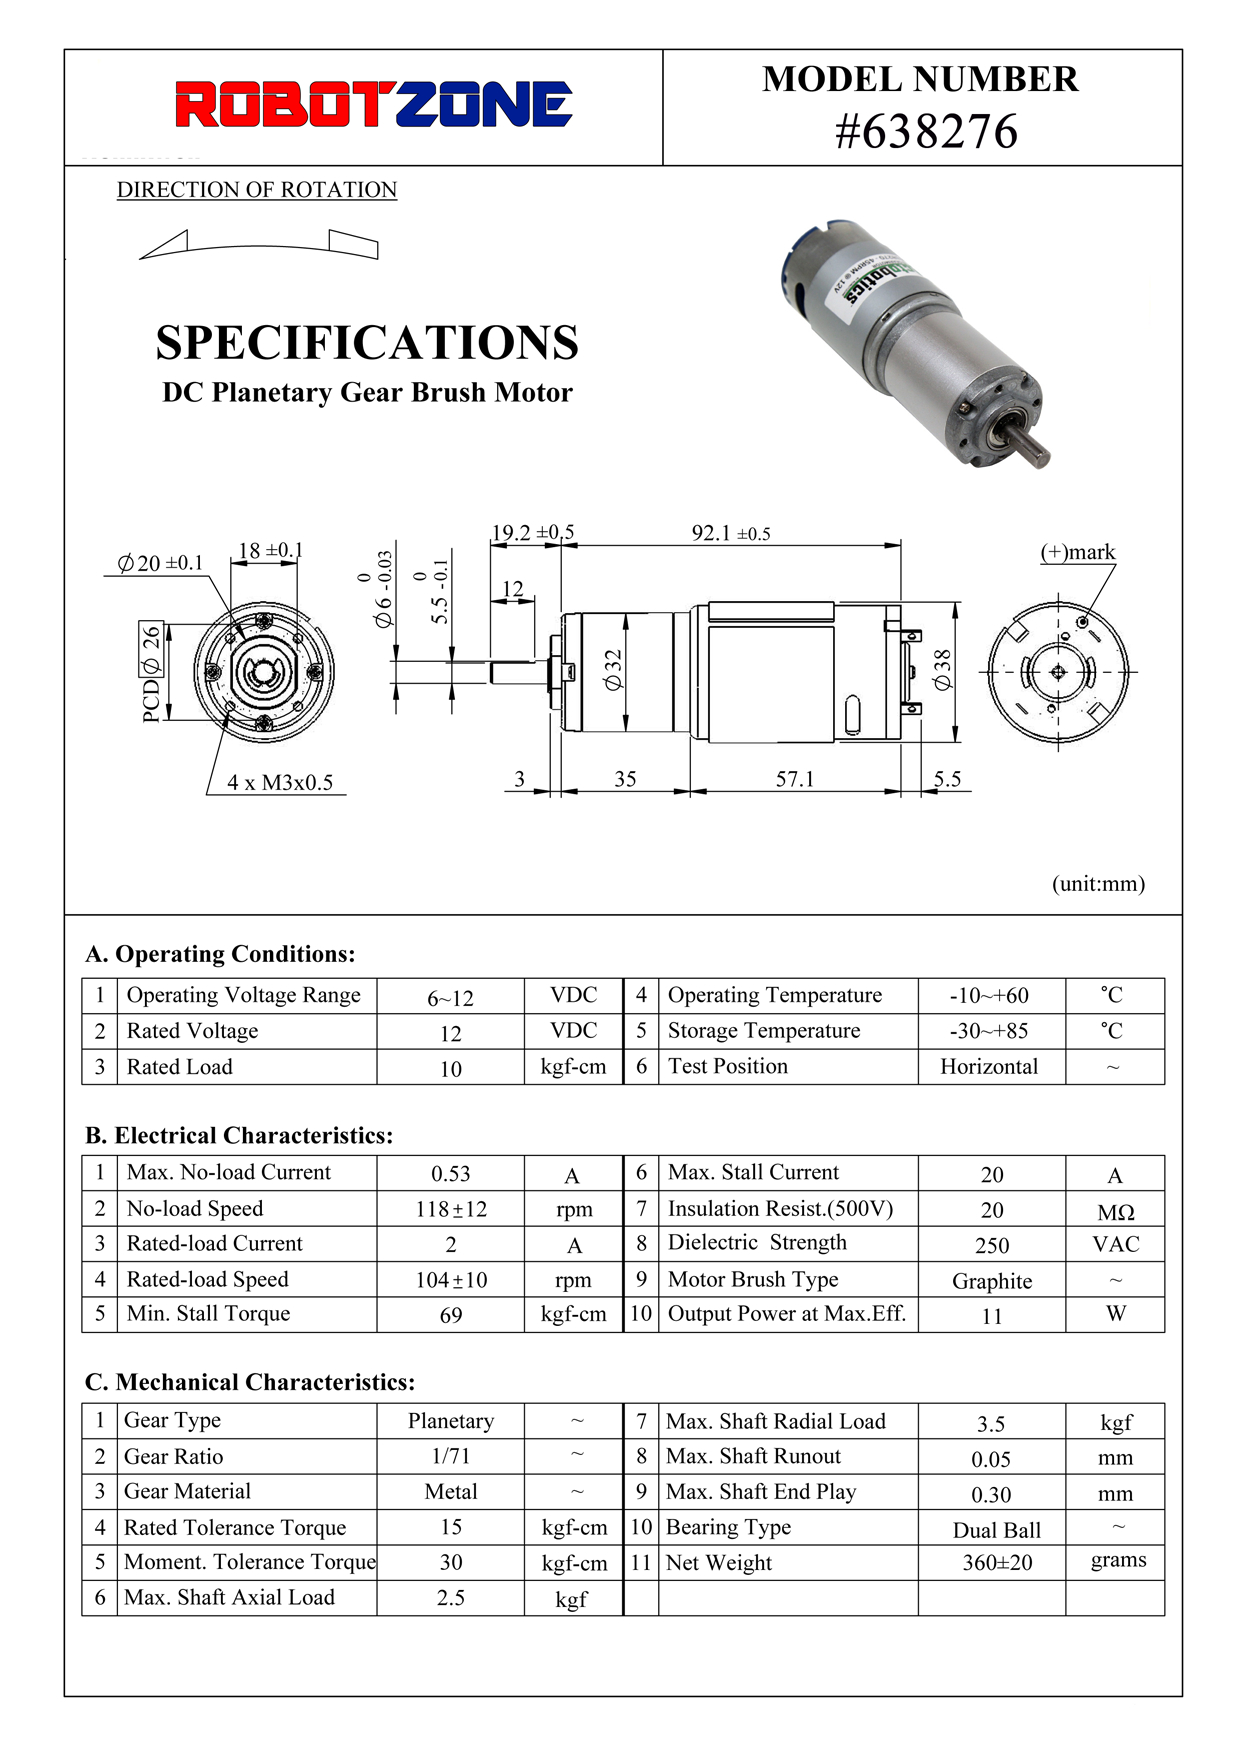
\includepdf[pages=1]{fabricante/servomotor.pdf}


%%% Local Variables:
%%% mode: latex
%%% TeX-master: t
%%% End:

\chapter{STM32F4 Encoder}

A continuación, las siguientes tres páginas representan la información contenida en el manual de usuario del stm32f411 con respecto a el funcionamiento de los encoders de cuadratura, y la configuración pertinente del lado del stm.

\includepdf[pages=277-279]{fabricante/rm0383.pdf}
%%% Local Variables:
%%% mode: latex
%%% TeX-master: t
%%% End:

\chapter{Roboclaw Instrucciones}

A continucación se muestran tres páginas con información relevante para la escritura de una librería de comunicación hacia el controlador de motores Roboclaw.

\includepdf[pages={64-65,70}]{fabricante/roboclaw_user_manual.pdf}

%%% Local Variables:
%%% mode: latex
%%% TeX-master: t
%%% End:

\backmatter

% 10. BILIOGRAFÍA
% --------------
\bibliographystyle{plain}
\bibliography{contenido/bibliografia.bib}

%%%%%%%%%%%%%%%%%%%
\end{document}
%%%%%%%%%%%%%%%%%%%
